\motto{Comment se fait-il que M.~Gauss ait osé vous faire dire que la plupart de vos théorèmes lui étaient connus et qu'il en avait fait la découverte dès 1808. Cet excès d'impudence n'est pas croyable de la part d'un homme qui a assez de mérite personnel pour n'avoir pas besoin de s'approprier les découvertes des autres.

--- Adrien-Marie Legendre\footnote{Adrien-Marie Legendre (1752--1833) was a French mathematician known for his foundational contributions to number theory, statistics, and mathematical analysis. Apart from his mathematical contributions, he also helped formalize the metric system during the French Revolution.}, in a letter to Jacobi in 1827}
\chapter{Test curves}
\label{chap:testcurve}

A geodesic ray $(\varphi_t)_{t\in[0,\infty)}$ in $\PSH(X,\theta)$ records the asymptotic behavior of singularities along a path of potentials. In this chapter we encode the same information in the dual variable $\tau$. Instead of recording the potential at time $t$, the Legendre transform records, for each slope $\tau$, the model potential determined by the part of the ray growing at least linearly with slope $\tau$. This produces a concave decreasing family $\tau\mapsto\Gamma_\tau$ of model potentials; more precisely, a test curve $\Gamma$ is a concave decreasing family $(\Gamma_\tau)_{\tau<\Gamma_{\max}}$ of model potentials in $\PSH(X,\theta)$.

The central result is a correspondence initiated by Ross and Witt Nystr\"om\footnote{Witt and Nystr\"om are both family names of a single person. Some Swedes have double family names. It should not be spelled as Witt-Nystr\"om as some people do in the literature.}. It is the pluripotential-theoretic analogue of Legendre duality: a test curve gives a geodesic ray by taking a Legendre transform, and a suitable geodesic ray gives back a test curve by the inverse transform. Thus test curves provide an intrinsic language for the singularity data carried by geodesic rays.

We first develop test curves as self-contained objects. In \cref{sec:tc} we introduce their basic properties, including independence of the auxiliary form, behavior under bimeromorphic morphisms, closedness in the parameter $\tau$, log-concavity of the mass function and the $P$-equivalence relation on test curves. The Ross--Witt Nystr\"om correspondence is proved in \cref{sec:RWN}, where the Legendre transform is shown to give a bijection between test curves and geodesic rays.

The later sections adapt this picture to the singularity types needed elsewhere in the book. In \cref{sec:Imodeltc} we develop the $\mathcal I$-model version of the theory, including the $\mathcal I$-envelope of a test curve, the transition from $P$-model to $\mathcal I$-model test curves, and the corresponding notion of maximal geodesic ray. Finally, \cref{sec:operationtc} studies sums, translations, maxima, suprema, infima and rescalings of test curves. These operations are needed in the non-Archimedean theory of \cref{chap:NApotential}, where test curves provide the analytic input for the construction of non-Archimedean potentials.

Throughout the chapter we freely use the convex-analytic results of \cref{chap:convex}. Those results are stated for convex functions; when they are applied to concave functions here, they are applied to the negatives.


\section{The notion of test curves}\label{sec:tc}

Let $X$ be a connected compact K\"ahler manifold of dimension $n$ and $\theta$ be a smooth closed real $(1,1)$-form on $X$ representing a big cohomology class.

Recall that the notion of model potentials is defined in \cref{def:modelpot}.
\begin{definition}\label{def:testcur}
    A \emph{test curve}\index{test curve} $\Gamma$ in $\PSH(X,\theta)$ consists of a real number $\Gamma_{\max}$ together with a map $(-\infty,\Gamma_{\max})\rightarrow \PSH(X,\theta)$ denoted by $\tau\mapsto \Gamma_{\tau}$ satisfying the following conditions:
    \begin{enumerate}
        \item\label{itm:def:testcur:1} The map $\tau\mapsto \Gamma_{\tau}$ is concave and decreasing;
        \item\label{itm:def:testcur:2} $P_{\theta}[\Gamma_{\tau}]=\Gamma_{\tau}$;
        \item\label{itm:def:testcur:3} the potential
        \begin{equation}\label{eq:Gammaminf}
        \Gamma_{-\infty}\coloneqq \uscsup[\tau<\Gamma_{\max}]\Gamma_{\tau}
        \end{equation}
        satisfies
        \[
        \int_X \left(\theta+\ddc \Gamma_{-\infty}\right)^n>0.
        \]
    \end{enumerate}
    Let $\phi\in \PSH(X,\theta)_{>0}$ be a model potential.
    The set of test curves $\Gamma$ with $\Gamma_{-\infty}=\phi$ is denoted by $\TC(X,\theta;\phi)$\index{$\TC(X,\theta;\phi)$}.

    The union of all $\TC(X,\theta;\phi)$'s for various model potentials $\phi\in \PSH(X,\theta)_{>0}$ is denoted by $\TC(X,\theta)_{>0}$\index{$\TC(X,\theta)_{>0}$}.
\end{definition}
By \ref{itm:def:testcur:2}, $\sup_{X}\Gamma_{\tau}=0$ for each $\tau<\Gamma_{\max}$. So $\Gamma_{-\infty}\in \PSH(X,\theta)$ by \cref{prop:pshfunction_closedseq}.

Thanks to \cref{cor:incseqnppcont} and \ref{itm:def:testcur:3}, there is $C<\Gamma_{\max}$ so that whenever $\tau<C$, we have $\Gamma_{\tau}\in \PSH(X,\theta)_{>0}$. Then it follows that $\Gamma_{-\infty}$ is a model potential by \cref{prop:incnetmodel}.

\begin{remark}\label{rmk:extendtestcur}
    Sometimes it is convenient to extend $\Gamma_{\tau}$ to $\tau\geq \Gamma_{\max}$ as well. This can be done as follows: for $\tau>\Gamma_{\max}$, we set $\Gamma_{\tau}\equiv -\infty$. For $\tau=\Gamma_{\max}$, we set
    \[
        \Gamma_{\tau}\coloneqq \inf_{\tau'<\Gamma_{\max}}\Gamma_{\tau'}\in \PSH(X,\theta).
    \]
    Note that $\Gamma_{\tau}\in \PSH(X,\theta)$ by \cref{cor:decreasingnetL1conv}.
\end{remark}

In general, for any $x\in X$, the map $\tau\mapsto \Gamma_{\tau}(x)$ falls into one of the following three categories:
\begin{enumerate}
    \item\label{itm:Gammataux_1} $\Gamma_{\tau}(x)\equiv -\infty$;
    \item\label{itm:Gammataux_2} $\Gamma_{\tau}(x)>-\infty$ for all $\tau\leq \Gamma_{\max}$;
    \item\label{itm:Gammataux_3} there is $\tau(x)\in (-\infty,\Gamma_{\max}]$ so that $\Gamma_{\tau}(x)>-\infty$ for all $\tau \in (-\infty,\tau(x))$, and $\Gamma_{\tau}(x)=-\infty$ for all $\tau\geq \tau(x)$.
\end{enumerate}
The last two possibilities are illustrated in \cref{fig:testcurve_pointwise}.

\begin{figure}[ht]
\centering
\resizebox{0.95\textwidth}{!}{%
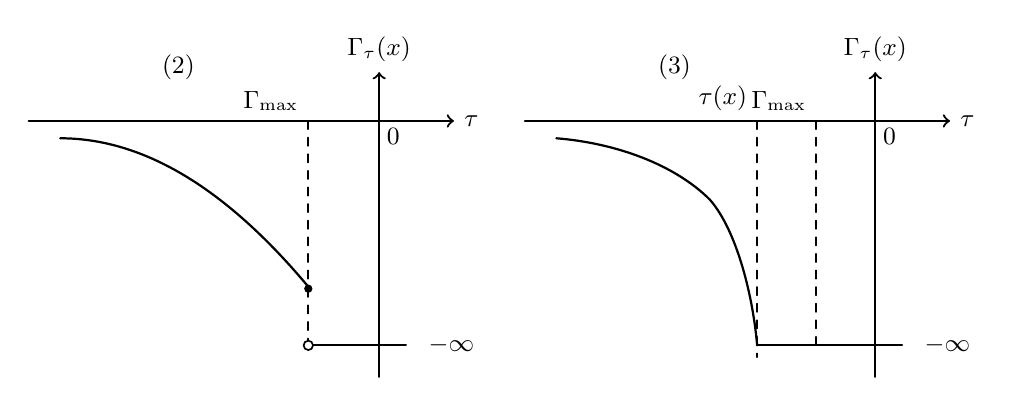
\begin{tikzpicture}[scale=1.0, line width=0.6pt, line cap=round, line join=round, every node/.style={font=\small}]
  \begin{scope}
    \draw[->, thick] (-4.45,0) -- (0.95,0) node[right] {$\tau$};
    \draw[->, thick] (0,-3.25) -- (0,0.62) node[above] {$\Gamma_\tau(x)$};
    \draw[thick] plot[smooth, samples=60, domain=-4.05:-0.90] (\x,{-0.22-0.19*(\x+4.05)*(\x+4.05)});
    \draw[dashed] (-0.90,0) -- (-0.90,-2.13);
    \draw[dashed] (-0.90,-2.13) -- (-0.90,-2.85);
    \draw[thick] (-0.90,-2.85) -- (0.34,-2.85);
    \fill (-0.90,-2.13) circle (1.5pt);
    \draw[fill=white] (-0.90,-2.85) circle (1.7pt);
    \node[above left] at (-0.90,0) {$\Gamma_{\max}$};
    \node[fill=white, inner sep=0.8pt] at (0.18,-0.20) {$0$};
    \node[right] at (0.50,-2.85) {$-\infty$};
    \node[above] at (-2.55,0.40) {(2)};
  \end{scope}

  \begin{scope}[xshift=6.3cm]
    \draw[->, thick] (-4.45,0) -- (0.95,0) node[right] {$\tau$};
    \draw[->, thick] (0,-3.25) -- (0,0.62) node[above] {$\Gamma_\tau(x)$};
    \draw[thick]
      (-4.05,-0.22)
      .. controls (-3.30,-0.28) and (-2.55,-0.55) .. (-2.10,-1.00)
      .. controls (-1.75,-1.40) and (-1.55,-2.25) .. (-1.50,-2.85);
    \draw[dashed] (-1.50,0) -- (-1.50,-3.0);
    \draw[dashed] (-0.75,0) -- (-0.75,-2.85);
    \draw[thick] (-1.50,-2.85) -- (0.34,-2.85);
    \node[above left] at (-1.50,0) {$\tau(x)$};
    \node[above left] at (-0.75,0) {$\Gamma_{\max}$};
    \node[fill=white, inner sep=0.8pt] at (0.18,-0.20) {$0$};
    \node[right] at (0.50,-2.85) {$-\infty$};
    \node[above] at (-2.55,0.40) {(3)};
  \end{scope}
\end{tikzpicture}
}
\caption{The last two pointwise possibilities for $\tau\mapsto\Gamma_\tau(x)$.}
\label{fig:testcurve_pointwise}
\end{figure}

Note that \ref{itm:Gammataux_2} is the generic situation. It occurs whenever $x\notin \{\Gamma_{\Gamma_{\max}}=-\infty\}$. In particular, when this situation occurs, $(-\infty,\Gamma_{\max})\ni \tau\mapsto \Gamma_{\tau}(x)$ is finite concave, and hence continuous. As a consequence, for any $\tau \in (-\infty,\Gamma_{\max})$, we have
\begin{equation}\label{eq:Gammataucont}
    \Gamma_{\tau}=\inf_{\tau'<\tau}\Gamma_{\tau'},\quad \Gamma_{\tau}=\uscsup[\tau'\in (\tau,\Gamma_{\max})]\Gamma_{\tau'}
\end{equation}
almost everywhere and hence everywhere due to \cref{prop:pshfuncdetdense}.

Recall that according to our general principle, we speak of model potentials only when a potential has positive mass. 
\begin{lemma}\label{lma:testcurvposmass}
Assume that $\Gamma\in \TC(X,\theta)_{>0}$. Then for each $\tau<\Gamma_{\max}$, we have
\begin{equation}\label{eq:dalethtauposmass}
\int_X \left(\theta+\ddc \Gamma_{\tau}\right)^n>0.
\end{equation}
In particular, $\Gamma_{\tau}$ is a model potential in $\PSH(X,\theta)_{>0}$.
\end{lemma}
The notations in the proof below are summarized in \cref{fig:tc}.
    \begin{figure}[ht]
\centering
\begin{tikzpicture}[scale=1.0, line width=0.6pt, every node/.style={font=\small}]
  % tau-axis
  \draw[->, thick] (-0.5,1.4) -- (8.0,1.4) node[right] {$\tau$};
  % Concave decreasing curve  y(t) = 1 - 0.05 (t+1)^2  for t in [-0.5,6.5]
  \draw[thick] plot[smooth, samples=80, domain=-0.5:6.5] (\x, {1 - 0.05*(\x+1)*(\x+1)});
  % At tau_max the curve drops to -infty
  \draw[thick, dashed] (6.5,-1.8) -- (6.5,-3.2);
  % Sample levels tau_0 < tau < tau'
  \pgfmathsetmacro{\Yz}{1-0.05*4}      % at tau_0=1
  \pgfmathsetmacro{\Ymid}{1-0.05*16}   % at tau=3
  \pgfmathsetmacro{\Yp}{1-0.05*36}     % at tau'=5
  \draw[red!75!black, dashed, thin] (1,1.4) -- (1,\Yz);
  \draw[red!75!black, dashed, thin] (3,1.4) -- (3,\Ymid);
  \draw[red!75!black, dashed, thin] (5,1.4) -- (5,\Yp);
  \draw[red!75!black, dashed, thin] (6.5,1.4) -- (6.5,-1.8);
  \node[red!75!black, above=2pt] at (1,1.4) {$\tau_0$};
  \node[red!75!black, above=2pt] at (3,1.4) {$\tau$};
  \node[red!75!black, above=2pt] at (5,1.4) {$\tau'$};
  \node[red!75!black, above=2pt] at (6.5,1.4) {$\tau_{\max}$};
  % Chord between Gamma_{tau_0} and Gamma_{tau'} (illustrates concavity)
  \draw[blue!70!black, thick] (1,\Yz) -- (5,\Yp);
  \fill[blue!70!black] (1,\Yz) circle (1.6pt);
  \fill[blue!70!black] (3,\Ymid) circle (1.6pt);
  \fill[blue!70!black] (5,\Yp) circle (1.6pt);
  % Label for the curve and for -infty drop
  \node[anchor=east] at (-0.5,0.95) {$\Gamma$};
  \node at (7.4,-2.6) {$-\infty$};
\end{tikzpicture}
\caption{The test curve $\Gamma$.}
\label{fig:tc}
\end{figure}

\begin{proof}

    Fix $\tau\in (-\infty,\Gamma_{\max})$.

    By assumption, $\Gamma_{-\infty}$ has positive mass. By \cref{cor:incseqnppcont}, we have
    \[
    \int_X \theta_{\Gamma_{-\infty}}^n=\lim_{\tau\to -\infty}\int_X \theta_{\Gamma_{\tau}}^n.
    \]
    In particular, for a sufficiently small $\tau_0<\tau$, we have
    \[
    \int_X \theta_{\Gamma_{\tau_0}}^n>0.
    \]
    Now take $\tau'\in (\tau, \Gamma_{\max})$ and $t\in (0,1)$ so that
    \[
    \tau=(1-t)\tau'+t\tau_0.
    \]
    From the concavity of $\Gamma$, we find that
    \[
    \Gamma_{\tau}\geq (1-t)\Gamma_{\tau'}+t\Gamma_{\tau_0}.
    \]
    By the monotonicity theorem \cref{thm:mono} and the multi-linearity of the non-pluripolar products \itemref{itm:prop:npp1:6},
    \[
    \int_X \theta_{\Gamma_{\tau}}^n\geq \int_X \theta_{(1-t)\Gamma_{\tau'}+t\Gamma_{\tau_0}}^n\geq t^n \int_X \theta_{\Gamma_{\tau_0}}^n>0
    \]
    and \eqref{eq:dalethtauposmass} follows.
\end{proof}

\begin{proposition}\label{prop:testcurvmasslogconc}
    Let $\Gamma\in \TC(X,\theta)_{>0}$. Then the map
    \[
    [-\infty,\Gamma_{\max})\rightarrow \mathbb{R},\quad \tau\mapsto \log \int_X \theta_{\Gamma_{\tau}}^n
    \]
    is continuous and concave on $(-\infty,\Gamma_{\max})$.
\end{proposition}
\begin{proof}
    The concavity of this function follows from \cref{thm:logconc} and \cref{thm:mono}. The continuity at $-\infty$ is a consequence of \cref{cor:incseqnppcont}.
    The continuity on $(-\infty,\Gamma_{\max})$ follows from the fact that finite concave functions on open intervals are continuous.
\end{proof}

\begin{definition}\label{def:relattestcurv}
    Let $\phi\in \PSH(X,\theta)_{>0}$ be a model potential.

    A test curve $\Gamma\in \TC(X,\theta;\phi)$ is said to be \emph{bounded}\index{test curve!bounded test curve} if for $\tau$ small enough, $\Gamma_{\tau}=\phi$. The subset of bounded test curves in $\TC(X,\theta;\phi)$ is denoted by $\TC^{\infty}(X,\theta;\phi)$\index{$\TC^{\infty}(X,\theta;\phi)$}.
    In this case, we write
    \begin{equation}\label{eq:Gammamin}
    \Gamma_{\min}\coloneqq \sup\{\tau\in \mathbb{R}:\Gamma_{\tau}=\phi\}.
    \end{equation}

    A test curve $\Gamma\in \TC(X,\theta;\phi)$ is said to have \emph{finite energy}\index{test curve!test curve with finite energy} if
    \begin{equation}\label{eq:tcfiniteenergy}
    \mathbf{E}^{\phi}(\Gamma)\coloneqq \Gamma_{\max} \int_X \theta_{\phi}^n+\int_{-\infty}^{\Gamma_{\max}} \left(\int_X\theta_{\Gamma_{\tau}}^n-\int_X \theta_{\phi}^n\right)\,\mathrm{d}\tau>-\infty.
    \end{equation}
    \index{$\mathbf{E}^{\phi}$}
    When $\phi=V_{\theta}$, we write $\mathbf{E}$ instead of $\mathbf{E}^{\phi}$.

    The subset of test curves with finite energy in $\TC(X,\theta;\phi)$ is denoted by $\TC^1(X,\theta;\phi)$\index{$\TC^1(X,\theta;\phi)$}.
\end{definition}

\begin{example}\label{ex:cantest}
    Given $\varphi\in \PSH(X,\theta)$, there is a canonically associated test curve $\Gamma^{\varphi}\in \TC^{\infty}(X,\theta;V_{\theta})$: Set $\Gamma^{\varphi}_{\max}=0$ and
    \[
    \Gamma^{\varphi}_{\tau}=
    \begin{cases}
        V_{\theta},&\textup{if }\tau\leq -1;\\
        P_{\theta}\left[ (1+\tau)\varphi-\tau V_{\theta} \right],& \textup{if }-1<\tau<0.
    \end{cases}
    \]
    Note that $\Gamma^{\varphi}$ is indeed a test curve, as follows from \cref{prop:Pconc}. Indeed, the concavity and monotonicity in $\tau$ follow from \cref{prop:Pconc}, and $\Gamma^\varphi_{-\infty}=V_\theta$ has positive mass.
\end{example}

We first observe that the notion of test curves does not really depend on the choice of $\theta$ within its cohomology class.
\begin{proposition}\label{prop:testcurveindeptheta}
    Let $\theta'$ be another smooth closed real $(1,1)$-form on $X$ representing the same cohomology class as $\theta$. Let $\phi\in \PSH(X,\theta)_{>0}$ be a model potential. Let $\phi'\in \PSH(X,\theta')_{>0}$ be the unique model potential satisfying $\phi\sim\phi'$.

    Then there is a canonical bijection
    \[
    \TC(X,\theta;\phi)\xrightarrow{\sim} \TC(X,\theta';\phi').
    \]
    This bijection induces the following bijections:
    \[
    \TC^1(X,\theta;\phi)\xrightarrow{\sim}\TC^1(X,\theta';\phi'),\quad \TC^{\infty}(X,\theta;\phi)\xrightarrow{\sim}\TC^{\infty}(X,\theta';\phi').
    \]
    These bijections satisfy the obvious cocycle conditions.
\end{proposition}
\begin{proof}
    Choose $g\in C^{\infty}(X)$ such that $\theta'=\theta+\ddc g$. Given any $\Gamma\in \TC(X,\theta;\phi)$, we observe that $\Gamma'\colon (-\infty,\Gamma_{\max})\rightarrow \PSH(X,\theta')$ defined as
    \[
    \tau\mapsto P_{\theta'}[\Gamma_{\tau}-g]
    \]
    lies in $\TC(X,\theta';\phi')$. In fact, the concavity and monotonicity of $\Gamma'$ follow from \cref{prop:Pconc}. Moreover, applying \cref{prop:incnetmodel} to the increasing net obtained as $\tau\to -\infty$ gives
    \[
        \Gamma'_{-\infty}=P_{\theta'}[\Gamma_{-\infty}-g]=P_{\theta'}[\phi-g]=\phi'.
    \]
    Thus $\Gamma'\in \TC(X,\theta';\phi')$.
    
    Moreover, the choice of $g$ is irrelevant since for any other choice of $g$, say $g'$, we have
    \[
    \Gamma_{\tau}-g\sim \Gamma_{\tau}-g'
    \]
    for all $\tau<\Gamma_{\max}$. The inverse construction is obtained by replacing $g$ with $-g$. The boundedness condition is clearly preserved. Finally, by \cref{prop:Ppresmass}, for every $\tau<\Gamma_{\max}$,
    \[
        \int_X(\theta'+\ddc \Gamma'_\tau)^n=\int_X(\theta+\ddc \Gamma_\tau)^n,
    \]
    and the same holds for $\phi$ and $\phi'$. Hence the finite energy condition is preserved. The cocycle condition is immediate from the uniqueness of the model representative in a fixed singularity type.
\end{proof}


\begin{proposition}\label{prop:ETCbimero}
    Let $\pi\colon Y\rightarrow X$ be a proper bimeromorphic morphism from a K\"ahler manifold $Y$. Then the pointwise pull-back induces a bijection
    \[
    \pi^*\colon \TC(X,\theta;\phi)\xlongrightarrow{\sim} \TC(Y,\pi^*\theta;\pi^*\phi).
    \]
\end{proposition}
\begin{proof}
     The bijectivity on the underlying potentials follows from \cref{prop:PSHpullbij}. The compatibility with model potentials follows from \cref{prop:Penvbimero}. These two facts also preserve concavity, monotonicity and the value of $\Gamma_{-\infty}$, hence give the asserted bijection of test curves.
\end{proof}

Next we verify the closedness of a test curve as a family of concave functions, so that no pathology arises in the Legendre transforms considered below. The notion of closedness is recalled in \cref{def:convexclosure}.
\begin{proposition}\label{prop:Gammaclosed}
    Let $\Gamma$ be a test curve in $\PSH(X,\theta)$. For each $x\in X$, the map $\mathbb{R} \ni\tau\mapsto \Gamma_{\tau}(x)$ is a closed concave function. Moreover, the map is proper as long as $\Gamma_{\Gamma_{\max}}(x)\neq -\infty$.
\end{proposition}

\begin{proof}
    We prove closedness.
    Fix $x\in X$. Assume that $\Gamma_{\tau}(x)\neq -\infty$ for some $\tau\in \mathbb{R}$. We only need to argue the upper semicontinuity of $\tau\mapsto \Gamma_{\tau}(x)$. The upper semicontinuity is clear at $\tau\geq \Gamma_{\max}$, so we are reduced to prove the following:
    \begin{equation}\label{eq:Gammatautemp1}
        \Gamma_{\tau}=\inf_{\tau'<\tau}\Gamma_{\tau'}
    \end{equation}
    for any $\tau<\Gamma_{\max}$. Take $\tau''\in (\tau,\Gamma_{\max})$. Outside the polar locus of $\Gamma_{\tau''}$, we know that \eqref{eq:Gammatautemp1} holds by continuity of real-valued concave functions. So \eqref{eq:Gammatautemp1} holds everywhere by \cref{prop:pshfuncdetdense}.

    The final assertion follows from properness of a finite closed concave function on its effective domain.
\end{proof}


\begin{definition}\label{def:Ptestcurve}
    Let $\Gamma\in \TC(X,\theta)_{>0}$ and $\omega$ be a smooth closed real positive $(1,1)$-form. Then we define
    $P_{\theta+\omega}[\Gamma]\in \TC(X,\theta+\omega)_{>0}$ as follows:
    \index{test curve!P-envelope@$P$-envelope of a test curve}
    \index{$P_{\theta+\omega}[\Gamma]$}
    \begin{enumerate}
        \item\label{itm:def:Ptestcurve:1} Define
        \[
        P_{\theta+\omega}[\Gamma]_{\max}=\Gamma_{\max};
        \]
        \item\label{itm:def:Ptestcurve:2} for each $\tau<\Gamma_{\max}$, define
        \[
        P_{\theta+\omega}[\Gamma]_{\tau}=P_{\theta+\omega}[\Gamma_{\tau}].
        \]
    \end{enumerate}
\end{definition}
It follows from \cref{prop:Pconc} that the family $P_{\theta+\omega}[\Gamma]$ is concave and decreasing. Moreover, since $\omega$ is positive,
\[
\int_X(\theta+\omega+\ddc\Gamma_\tau)^n \geq \int_X(\theta+\ddc\Gamma_\tau)^n>0
\]
for every $\tau<\Gamma_{\max}$, and hence $P_{\theta+\omega}[\Gamma]_\tau$ is a model potential by \cref{cor:Psendspotentialtomodel}. Thus $P_{\theta+\omega}[\Gamma]\in\TC(X,\theta+\omega)_{>0}$.

\begin{proposition}\label{prop:PpreGammainf}
    Let $\Gamma\in \TC(X,\theta)_{>0}$ and $\omega$ be a closed real smooth positive $(1,1)$-form on $X$. Then
    \[
    P_{\theta+\omega}[\Gamma]_{-\infty}=P_{\theta+\omega}[\Gamma_{-\infty}].
    \]
\end{proposition}
\begin{proof}
     This follows from \cref{prop:incnetmodel}.
\end{proof}

\section{Ross--Witt Nystr\"om correspondence}\label{sec:RWN}
Let $X$ be a connected compact K\"ahler manifold of dimension $n$ and $\theta$ be a smooth closed real $(1,1)$-form on $X$ representing a big cohomology class.
Fix a model potential $\phi\in \PSH(X,\theta)_{>0}$.

\cref{prop:Gammaclosed} allows us to talk about the Legendre transforms of test curves in the expected way.

The general definition of the Legendre transform \cref{def:Legendregeneral} can be translated as follows:
\begin{definition}\label{def:Legtrans}
    Let $\Gamma\in \TC(X,\theta;\phi)$. We define its \emph{Legendre transform}\index{Legendre transform} as the map $\Gamma^*\colon (0,\infty)\rightarrow \PSH(X,\theta)$ given by
    \begin{equation}\label{eq:testcurveLegtran}
        \Gamma^*_t=\sup_{\tau\in \mathbb{R}} \left(t\tau+ \Gamma_{\tau}\right)\footnotemark.
    \end{equation}
    \footnotetext{There is no usc regularization in the preceding formula. This is not a typo.}
\end{definition}
Thanks to \cref{rmk:extendtestcur}, \eqref{eq:testcurveLegtran} can be equivalently written as
\[
\Gamma^*_t=\sup_{\tau<\Gamma_{\max}} \left(t\tau+ \Gamma_{\tau}\right)=\sup_{\tau\leq \Gamma_{\max}} \left(t\tau+ \Gamma_{\tau}\right).
\]


It is sometimes handy to \emph{define}
\begin{equation}\label{eq:Gamma0star}
\Gamma^*_0\coloneqq \phi
\end{equation}
at $t=0$. But it is important to remember that, with this convention, \eqref{eq:testcurveLegtran} is not true at $t=0$ in general.

\begin{remark}\label{rmk:negativeray}
Here we do not discuss the case $t<0$ because its behavior is straightforward: take $x\in X$; if $\Gamma_{\tau}(x)=-\infty$ for all $\tau<\Gamma_{\max}$, then $\Gamma_t^*(x)=-\infty$; otherwise, $\Gamma_t^*(x)=\infty$.
\end{remark}

The information about $t>0$ suffices to characterize $\Gamma$.
\begin{proposition}\label{prop:Leginvtc}
    Let $\Gamma\in \TC(X,\theta;\phi)$. Then
    \begin{equation}\label{eq:Leginvtc}
    \Gamma_{\tau}=\inf_{t>0} \left(\Gamma^*_t-t\tau\right)
    \end{equation}
    for all $\tau\in \mathbb{R}$.
\end{proposition}
Due to our convention \eqref{eq:Gamma0star}, in \eqref{eq:Leginvtc} we may equivalently take $t\geq 0$.
\begin{proof}
    Fix $x\in X$. We want to establish \eqref{eq:Leginvtc} at $x$.
    We distinguish two cases. First suppose that $\Gamma_{\tau}(x)=-\infty$ for all $\tau<\Gamma_{\max}$ and hence all $\tau\in \mathbb{R}$. In this case, we have $\Gamma_t^*(x)=-\infty$ for all $t>0$. Therefore, \eqref{eq:Leginvtc} follows trivially.

    Otherwise, by \cref{rmk:negativeray}, we know that $\Gamma^*_t(x)=\infty$ for all $t<0$. The relative interior of the domain of $t\mapsto \Gamma^*_t(x)$ is contained in $(0,\infty)$.
    Therefore, \eqref{eq:Leginvtc} follows from \cref{thm:Legendredual}, \cref{prop:Gammaclosed}.
\end{proof}

In \cref{def:Legtrans}, we made the nontrivial claim that $\Gamma^*_t\in \PSH(X,\theta)$ for all $t>0$. Let us prove this.
\begin{lemma}\label{lma:testcurvelegusc}
    Let $\Gamma\in \TC(X,\theta;\phi)$. Then $\Gamma^*_t\in \PSH(X,\theta)$ for all $t>0$. In fact, $\Gamma^*$ is upper semicontinuous as a function of $X\times (0,\infty)$.
\end{lemma}
\begin{proof}
    We first observe that for each $x\in X$, we have
    \[
        \Gamma_t^*(x)\leq t\Gamma_{\max}<\infty.
    \]

    Let $R=\{a+\mathrm{i}b\in \mathbb{C}:a>0,b\in \mathbb{R}\}$. We consider
    \[
        F\colon X\times R\rightarrow [-\infty,\infty),\quad (x,a+\mathrm{i}b)\mapsto \Gamma_a^*(x).
    \]
    Let $\pi\colon X\times R\rightarrow X$ be the natural projection.
    Observe that the upper semicontinuous regularization $G$ of $F$ is $\pi^*\theta$-psh by \cref{prop:pshfunction_closedseq}.
    It suffices to show that $F=G$.
    We let
    \[
        E\coloneqq \left\{ (x,z)\in X\times R: F(x,z)<G(x,z)  \right\}.
    \]
    We want to argue that $E=\varnothing$. Since $F$ is invariant under translations in the imaginary direction of $R$, the same is true for its upper semicontinuous regularization $G$. So $E$ can be written as $B\times \mathrm{i}\mathbb{R}$ for some set $B\subseteq X\times (0,\infty)$. Since $E$ is a pluripolar set by \cref{prop:supsupstardiff}, it has zero Lebesgue measure. Hence, $B$ has zero Lebesgue measure. For each $x\in X$, write
    \[
        B_x=\left\{t\in (0,\infty): (x,t)\in B \right\}.
    \]
    By Fubini's theorem, $B_x$ has vanishing $1$-dimensional Lebesgue measure for all $x\in X\setminus Z$, where $Z\subseteq X$ is a subset of measure $0$. We may assume that $Z\supseteq \{\Gamma_{\Gamma_{\max}}=-\infty\}$ so that for $x\in X\setminus Z$, $\Gamma^*_t(x)\neq -\infty$ for all $t>0$.

    For any $x\in X\setminus Z$, both $t\mapsto F(x,t)$ and $G(x,t)$ are convex functions with values in $\mathbb{R}$ on $(0,\infty)$. They agree almost everywhere, hence everywhere by their continuity. It follows that for $x\in X\setminus Z$, we have $B_x=\varnothing$.

    By \cref{prop:Leginvtc}, for any $x\in X$, we have
    \[
        \Gamma_{\tau}(x)=\inf_{t>0} (F(x,t)-t\tau),\quad \tau<\Gamma_{\max}.
    \]
    On the other hand, let
    \begin{equation}\label{eq:chiGlegtemp1}
        \chi_{\tau}(x)=\inf_{t>0} (G(x,t)-t\tau),\quad \tau<  \Gamma_{\max},\quad x\in X.
    \end{equation}
    By Kiselman's principle \cref{prop:Kis}, $\chi_{\tau}\in \PSH(X,\theta)$. But on $X\setminus Z$, we already know that $\Gamma_{\tau}=\chi_{\tau}$ for all $\tau<\Gamma_{\max}$. By \cref{prop:pshfuncdetdense},
    \[
    \Gamma_{\tau}=\chi_{\tau},\quad \tau<\Gamma_{\max}.
    \]
    Now we conclude that $F(x,t)=G(x,t)$ by \cref{cor:Leginvpartdef}.
\end{proof}

\begin{corollary}\label{cor:GammastarP}
    Let $\Gamma \in \TC(X,\theta;\phi)$. Then $\Gamma^*_t\in \mathcal{E}(X,\theta;\phi)$ for all $t>0$.
\end{corollary}
\begin{proof}
Fix $t>0$.
    We already know that $\Gamma^*_t\in \PSH(X,\theta)$ by \cref{lma:testcurvelegusc}. It suffices to show that
    \[
    \Gamma^*_t\sim_P \phi.
    \]
    From \eqref{eq:testcurveLegtran} and \cref{prop:Ppartialsup}, we know that
    \[
    \Gamma^*_t\sim_P \uscsup[\tau<\Gamma_{\max}] \Gamma_{\tau}=\phi.
    \]
    This completes the proof.
\end{proof}

\begin{lemma}\label{lma:suplegenlinear}
    Let $\Gamma\in \TC(X,\theta;\phi)$. Then
    \[
        \sup_X \Gamma_t^*=t\Gamma_{\max}
    \]
    for all $t>0$.

    In particular, $t\mapsto \Gamma^*_t-t\Gamma_{\max}$ is a decreasing function in $t>0$.
\end{lemma}
\begin{proof}
    Since $\Gamma_{\tau}\leq 0$ for all $\tau<\Gamma_{\max}$, we have
    \[
        \sup_X \Gamma_t^*\leq t\Gamma_{\max}
    \]
    for all $t>0$.
    Conversely, for each $\tau<\Gamma_{\max}$,
    \[
        \sup_X\Gamma_t^*\geq \sup_X(t\tau+\Gamma_{\tau})=t\tau.
    \]
    Letting $\tau\to\Gamma_{\max}$ gives the reverse inequality.
    The final assertion follows directly from the formula
    \[
        \Gamma_t^*-t\Gamma_{\max}=\sup_{\tau<\Gamma_{\max}}\Bigl(\Gamma_\tau-t(\Gamma_{\max}-\tau)\Bigr).
    \]
    This completes the proof.
\end{proof}

\begin{lemma}\label{lma:LegsendsTCtoR}
    Given $\Gamma\in \TC(X,\theta;\phi)$, we have $\Gamma^*\in \mathcal{R}(X,\theta;\phi)$.
\end{lemma}
See \cref{def:geodraydef} for the notation $\mathcal{R}(X,\theta;\phi)$.
\begin{proof}
    It follows from \cref{lma:testcurvelegusc}, \eqref{eq:testcurveLegtran} and \cref{prop:pshfunction_closedseq} that the restriction of $\Gamma^*$ to each compact subinterval of $(0,\infty)$ is a subgeodesic. By \cref{cor:GammastarP}, for any $t>0$, $\Gamma^*_t\in \mathcal{E}(X,\theta;\phi)$.

    First observe that as $t\to 0+$, we have
    \begin{equation}\label{eq:GammatophiL1temp}
        \Gamma_t^*\xrightarrow{L^1}\phi.
    \end{equation}
    By \cref{lma:suplegenlinear} and \cref{prop:L1compa}, it suffices to show each $L^1$-cluster point $\psi\in \PSH(X,\theta)$ of $\Gamma_t^*$ as $t\to 0$ is equal to $\phi$.

    To see this, first observe that by \eqref{eq:testcurveLegtran}, for any fixed $t>0$,
    \[
        \Gamma_t^*\leq t\Gamma_{\max}+\phi.
    \]
    Therefore, $\psi\leq \phi$. On the other hand, for any fixed $\tau<\Gamma_{\max}$, by \eqref{eq:testcurveLegtran}, we have
    \[
        \Gamma^*_t\geq \Gamma_{\tau}+t\tau
    \]
    for any $t>0$. So $\psi\geq \Gamma_{\tau}$ almost everywhere and hence everywhere by \cref{prop:pshfuncdetdense}. It follows that $\psi\geq \phi$. Therefore, $\psi=\phi$.

     Assume that $\Gamma^*$ is not a geodesic ray. Then we can find $0\leq a<b$ such that $(\Gamma^*_t)_{t\in (a,b)}$ differs from the geodesic $(\eta_t)_{t\in (a,b)}$ from $\Gamma^*_a$ to $\Gamma^*_b$. The existence of $(\eta_t)_t$ is guaranteed by \cref{prop:perronenvissubgeod}.
     We consider the subgeodesic $(\ell_t)_{t>0}$ given by $\ell_t=\eta_t$ for $t\in (a,b)$ and $\ell_t=\Gamma^*_t$ otherwise. Note that $\ell$ is a subgeodesic due to the gluing lemma \cref{lma:subgeodgluing}.

     Consider the Legendre transform
    \[
        \Gamma'_{\tau}=\inf_{t>0} (\ell_t-t\tau),\quad \tau\in \mathbb{R}.
    \]
    Then $\Gamma'_{\tau}\geq \Gamma_{\tau}$ and $\Gamma'_{\tau}\in \PSH(X,\theta)\cup\{-\infty\}$ by \cref{prop:Kis} for all $\tau\in \mathbb{R}$.

    We claim that
    \begin{equation}\label{eq:GammapGammcomptemp1}
        \Gamma'_{\tau}\leq \Gamma_{\tau}+(b-a)(\Gamma_{\max}-\tau),\quad \tau\in \mathbb{R}.
    \end{equation}
    Observe that $\Gamma'_{\tau}\equiv -\infty$ when $\tau>\Gamma_{\max}$ by \cref{lma:suplegenlinear}. Thus it suffices to consider $\tau\leq \Gamma_{\max}$. Put
    \[
        C_{\tau}\coloneqq (b-a)(\Gamma_{\max}-\tau)\geq 0.
    \]
    For any $s\in [a,b]$, the monotonicity of $t\mapsto \Gamma_t^*-t\Gamma_{\max}$ from \cref{lma:suplegenlinear} gives
    \[
        \Gamma_b^*-b\tau \leq \Gamma_s^*-s\tau+C_{\tau}.
    \]
    Since $\ell_b=\Gamma_b^*$, we get
    \[
        \Gamma'_{\tau}\leq \Gamma_b^*-b\tau\leq \Gamma_s^*-s\tau+C_{\tau},\quad s\in [a,b].
    \]
    For $s\notin [a,b]$, we have $\ell_s=\Gamma_s^*$, hence
    \[
        \Gamma'_{\tau}\leq \Gamma_s^*-s\tau\leq\Gamma_s^*-s\tau+C_{\tau}.
    \]
    Taking the infimum over all $s>0$ gives
    \[
        \Gamma'_{\tau}\leq \Gamma_{\tau}+C_{\tau}.
    \]
    Therefore, \eqref{eq:GammapGammcomptemp1} follows.
    In particular, for any $\tau<\Gamma_{\max}$, we have $\Gamma'_{\tau}\sim \Gamma_{\tau}$.
    Moreover, $\sup_X\ell_t\leq t\Gamma_{\max}$ for all $t>0$: this is clear outside $(a,b)$ from \cref{lma:suplegenlinear}, and on $(a,b)$ it follows from the convexity of subgeodesics applied to the geodesic $(\eta_t)_{t\in(a,b)}$. Hence, for $\tau<\Gamma_{\max}$,
    \[
        \sup_X(\ell_t-t\tau)\leq t(\Gamma_{\max}-\tau).
    \]
    Letting $t\to 0+$ gives $\Gamma'_{\tau}\leq 0$. It follows from the fact that $\Gamma_{\tau}$ is a model potential that $\Gamma_{\tau}=\Gamma'_{\tau}$ for all $\tau<\Gamma_{\max}$. Therefore, by \cref{thm:Legendredual}, we have $\Gamma^*_t=\ell_t$ for all $t>0$, which is a contradiction.
\end{proof}
Given $\ell\in \mathcal{R}(X,\theta;\phi)$, define its Legendre transform
    \begin{equation}\label{eq:invLeg}
        \ell^*_{\tau}\coloneqq \inf_{t>0} (\ell_t-t\tau),\quad \tau \in \mathbb{R}.
    \end{equation}

\begin{lemma}\label{lma:LegendsRtoTC}
    Given $\ell\in \mathcal{R}(X,\theta;\phi)$, then $\ell^*=(\ell^*_\tau)_{\tau<\sup_X \ell_1}\in \TC(X,\theta;\phi)$.
\end{lemma}
\begin{proof}
    Note that it follows from \cref{prop:Kis} that $\ell^*_{\tau}\in \PSH(X,\theta)\cup \{-\infty\}$ for all $\tau\in \mathbb{R}$. It is clear that $\mathbb{R}\ni \tau\mapsto \ell^*_{\tau}$ is a decreasing and concave function.

    By \cref{prop:raysuplinear},
    \[
    \sup_X\ell_t= t\sup_X \ell_1 \quad \forall t\geq 0.
    \]
    Set $C=\sup_X\ell_1$. By \cref{prop:raysuplinear}, $\sup_X(\ell_t-Ct)=0$ for all $t>0$. For each $x$ outside a pluripolar set, the function $t\mapsto \ell_t(x)-Ct$ is convex on $(0,\infty)$ and bounded above by $0$, hence it is decreasing. By \cref{prop:pshfuncdetdense}, the same monotonicity holds as an inequality of $\theta$-psh functions. Thus $(\ell_t-Ct)_{t>0}$ is a decreasing net in $\PSH(X,\theta)$.

    Its infimum is not identically $-\infty$, since the family is normalized by $\sup_X(\ell_t-Ct)=0$ and is compact in $L^1$ by \cref{prop:L1compa}. Therefore
    \[
        \ell^*_{C}=\inf_{t>0}(\ell_t-Ct)\in \PSH(X,\theta)
    \]
    by \cref{prop:pshfunction_closedseq}.

    On the other hand, for $\tau>\sup_X \ell_1$, the same argument shows that
    \[
    \ell^*_{\tau}\equiv -\infty.
    \]
    Therefore, $\ell^*_{\tau}\in \PSH(X,\theta)$ if and only if $\tau\leq \ell^*_{\max}\coloneqq \sup_X \ell_1$.

    We claim that $(\ell^*_{\tau})_{\tau<\ell^*_{\max}}$ is a test curve. We first observe that for $\tau<\ell^*_{\max}$, we have
    \[
    \ell^*_{\tau}\leq \ell_1-\tau\sim_P \phi.
    \]
    Therefore,
    \begin{equation}\label{eq:elltaupreceqpphi}
        \ell^*_{\tau}\preceq_P \phi,\quad \forall \tau<\ell^*_{\max}.
    \end{equation}
    Also observe that for any $\tau\leq \ell^*_{\max}$ and any $t>0$, we have
    \[
    \sup_X \ell^*_{\tau}\leq \sup_X \ell_t-t\tau=\ell^*_{\max}t-t\tau.
    \]
    Letting $t\to 0+$, we find that for any $\tau\leq \ell^*_{\max}$, we have
    \begin{equation}\label{eq:supXelltaustarnegtemp1}
    \sup_X \ell^*_{\tau}\leq 0.
    \end{equation}

    Fix $\tau<\ell^*_{\max}$. We want to argue that
    \begin{equation}\label{eq:Pellstartemp1}
        P_{\theta}\left[\ell^*_{\tau}\right]=\ell^*_{\tau}.
    \end{equation}
    First we claim that for any $C>0$, we have
    \begin{equation}\label{eq:ellstartaupCtemp1}
    (\ell^*_{\tau}+C)\land \phi=(\ell^*_{\tau}+C)\land V_{\theta}.
    \end{equation}
    The $\leq$ direction is trivial. We argue the reverse inequality, which reduces to
    \[
     \phi\geq (\ell^*_{\tau}+C)\land V_{\theta}.
    \]
    Since $\phi$ is model and $(\ell^*_{\tau}+C)\land V_{\theta}\leq 0$, it suffices to show that
    \[
    \phi\succeq_P (\ell^*_{\tau}+C)\land V_{\theta},
    \]
    which follows from \eqref{eq:elltaupreceqpphi}. Therefore, \eqref{eq:ellstartaupCtemp1} is established. Thanks to \eqref{eq:supXelltaustarnegtemp1}, we have the obvious inequality
    \[
    (\ell^*_{\tau}+C)\land V_{\theta}\geq \ell^*_{\tau}
    \]
    for any $C>0$. Therefore, in order to prove \eqref{eq:Pellstartemp1}, it remains to argue that for any $C>0$,
    \begin{equation}\label{eq:ellstarleqetemp1}
        (\ell^*_{\tau}+C)\land \phi\leq  \ell^*_{\tau}.
    \end{equation}
    For this purpose, let us consider the following geodesics: For any $M>0$ and $t\in [0,1]$, let
    \[
        \ell^{1,M}_t= \ell_{tM}-tM\tau,\quad  \ell^{2,M}_t= (\ell^*_{\tau}+C)\land \phi-Ct.
    \]
    It is clear that at $t=0,1$, we have $\ell^{2,M}_t\leq \ell^{1,M}_t$. Hence, the same holds for all $t\in [0,1]$. In particular, for any fixed $s\in (0,1]$, we have
    \[
        (\ell^*_{\tau}+C)\land \phi-Cs\leq \ell_{sM}-sM\tau
    \]
    for all $M>0$.
    Taking infimum with respect to $M>0$, we find
    \[
        (\ell^*_{\tau}+C)\land \phi-Cs\leq \ell^*_{\tau}.
    \]
    Since $s\in (0,1]$ is arbitrary, we conclude \eqref{eq:ellstarleqetemp1}.

    Finally, we check the condition at $-\infty$. Set
    \[
        \psi\coloneqq \uscsup[\tau<\ell^*_{\max}]\ell^*_{\tau}.
    \]
    The family $(\ell^*_{\tau})_{\tau<\ell^*_{\max}}$ is locally uniformly bounded from above, so $\psi\in\PSH(X,\theta)$. Thanks to \cref{cor:subgeodboundary}, outside a pluripolar set, the function $t\mapsto \ell_t(x)$ is a finite closed convex function on $[0,\infty)$ with value $\phi(x)$ at $t=0$.
    Applying the one-variable Legendre duality gives
    \[
        \psi(x)=\adjustlimits \sup_{\tau<\ell^*_{\max}}\inf_{t>0}\bigl(\ell_t(x)-t\tau\bigr)=\ell_0(x)=\phi(x)\quad \textup{quasi-everywhere}.
    \]
    Hence $\psi=\phi$ by \cref{prop:pshfuncdetdense}. In particular, $\ell^*_{-\infty}=\phi$ has positive mass.
\end{proof}


\begin{theorem}\label{thm:Legenbij}
    The Legendre transform in \cref{def:Legtrans} is a bijection
    \begin{equation}\label{eq:RWNco}
        \TC(X,\theta;\phi)\xrightarrow{\sim} \mathcal{R}(X,\theta;\phi).
    \end{equation}
    Moreover, this bijection restricts to the following bijections:
    \begin{equation}\label{eq:RWNcotwocases}
    \TC^1(X,\theta;\phi)\xrightarrow{\sim} \mathcal{R}^1(X,\theta;\phi),\quad \TC^{\infty}(X,\theta;\phi)\xrightarrow{\sim} \mathcal{R}^{\infty}(X,\theta;\phi).
    \end{equation}
    For any $\Gamma\in \TC^1(X,\theta;\phi)$, we have
    \begin{equation}\label{eq:RWNenergy}
    \mathbf{E}^{\phi}(\Gamma)=\mathbf{E}^{\phi}(\Gamma^*).
    \end{equation}
\end{theorem}
Recall that the two energy functionals in \eqref{eq:RWNenergy} are defined in \eqref{eq:tcfiniteenergy} and \cref{def:radialMAenergy2} respectively.

The correspondence \eqref{eq:RWNco} will be referred to as the \emph{Ross--Witt Nyström correspondence}\index{Ross--Witt Nyström correspondence}.

To appreciate this result, just consider the simple case where $\theta$ is a Kähler form and $\phi=0$. In this case, elements in $\mathcal{R}^{\infty}(X,\theta)$ are rays of \emph{bounded} potentials, while elements in $\TC^{\infty}(X,\theta)$ are rays of \emph{singular} potentials. This result establishes a bridge between the pluripotential theory of regular potentials and that of singular potentials!

\begin{proof}
    \textbf{Step~1}. We first establish \eqref{eq:RWNco}.

    It follows from \cref{lma:LegsendsTCtoR} that the forward map is well-defined. The inverse map is given by \eqref{eq:invLeg}. We show that the inverse map is also well-defined. Given $\ell\in \mathcal{R}(X,\theta;\phi)$, we know from \cref{lma:LegendsRtoTC} that $\ell^*\in \TC(X,\theta;\phi)$.
    We need to show that $\ell^*\in \TC(X,\theta;\phi)$.

    The equality $\ell^*_{-\infty}=\phi$ was proved in \cref{lma:LegendsRtoTC}. Therefore, $\ell^*\in \TC(X,\theta;\phi)$ as expected.

    The two operations are inverse to each other thanks to \cref{cor:Leginvpartdef}. Hence, \eqref{eq:RWNco} is established.

    \textbf{Step~2}.
    Next we consider the bounded situation. Namely, we want to establish the second half of \eqref{eq:RWNcotwocases}.

    Suppose that $\Gamma\in \TC^{\infty}(X,\theta;\phi)$. Take $\tau_0\in \mathbb{R}$ so that $\Gamma_{\tau}=\phi$ for all $\tau\leq \tau_0$. It follows from \eqref{eq:testcurveLegtran} that
    \[
    \Gamma_t^*\geq \phi+t\tau_0
    \]
    for all $t>0$. Therefore, $\Gamma^*_t\sim \phi$ for all $t>0$ and hence $\Gamma^*\in \mathcal{R}^{\infty}(X,\theta;\phi)$.

    Conversely, suppose that $\ell\in \mathcal{R}^{\infty}(X,\theta;\phi)$. Thanks to \cref{prop:geodinfsublinear}, there is a constant $C>0$ such that
    \[
    \ell_t\geq \phi-Ct.
    \]
    Therefore, according to \eqref{eq:invLeg}, we have
    \[
    \ell^*_{\tau}\geq \inf_{t>0} \Bigl( \phi-(C+\tau)t \Bigr)=\phi
    \]
    if $\tau\leq -C$. Therefore, $\ell^*_{\tau}=\phi$ for all $\tau\leq -C$.

    \textbf{Step~3}. We establish \eqref{eq:RWNenergy} and the first half of \eqref{eq:RWNcotwocases}.

    \textbf{Step~3.1}. We reduce to the case where $\Gamma_{\max}=0$.

    Suppose that we define
    \[
    \Gamma'_{\tau}=\Gamma_{\tau+\Gamma_{\max}},\quad \forall \tau<0.
    \]
    Then $\Gamma'\in \TC(X,\theta;\phi)$ as well and for all $t>0$,
    \[
    \Gamma'^*_t=\sup_{\tau<0} \left( t\tau+\Gamma'_{\tau} \right)=\sup_{\tau<\Gamma_{\max}} \left( t\tau+\Gamma_{\tau} \right)-t\Gamma_{\max}=\Gamma^*_t-t\Gamma_{\max}.
    \]
    Therefore,
    \[
    \mathbf{E}^{\phi}\left(\Gamma'^*\right)=\mathbf{E}^{\phi}\left(\Gamma^*\right)-\Gamma_{\max}\int_X \theta_{\phi}^n.
    \]
    by \eqref{eq:Ephiaddcst}. Using \eqref{eq:tcfiniteenergy}, we also have
    \[
    \begin{aligned}
    \mathbf{E}^{\phi}(\Gamma')=&\int_{-\infty}^0 \left( \int_X \theta_{\Gamma'_{\tau}}^n-\int_X \theta_{\phi}^n \right)\,\mathrm{d}\tau\\
    =& \int_{-\infty}^{\Gamma_{\max}}\left( \int_X \theta_{\Gamma_{\tau}}^n-\int_X \theta_{\phi}^n \right)\,\mathrm{d}\tau\\
    =& \mathbf{E}^{\phi}(\Gamma)-\Gamma_{\max}\int_X \theta_{\phi}^n.
    \end{aligned}
    \]
    Therefore, it suffices to establish \eqref{eq:RWNenergy} for $\Gamma'$ in place of $\Gamma$.

    \textbf{Step~3.2}. We assume that $\Gamma_{\max}=0$ and $\Gamma\in \TC^{\infty}(X,\theta;\phi)$. We prove \eqref{eq:RWNenergy}.

    For $N\in \mathbb{Z}_{>0}$, $M \in \mathbb{Z}$, we introduce the following:
    \[
        \Gamma^{*,N,M}_t \coloneqq \max_{\substack{k \in \mathbb{Z} \\ k \leq M}} \left(\Gamma_{k/2^N} +  tk/2^N\right)\in \mathcal{E}^{\infty}(X,\theta;\phi),\quad t>0.
    \]
    We first claim that for all $t>0$, $N\in \mathbb{Z}_{>0}$ and $M\in \mathbb{Z}_{<0}$,
    \begin{equation}\label{eq:diff_eq_I}
        \frac{t}{2^N} \int_X \theta^n_{\Gamma_{(M+1)/2^N}}\leq E_{\theta}^{\phi}\left(\Gamma_t^{*,N,M+1}\right)-E_{\theta}^{\phi}\left(\Gamma_t^{*,N,M}\right)\leq \frac{t}{2^N} \int_X \theta^n_{\Gamma_{M/2^N}}.
    \end{equation}

    Assuming this, let us prove \eqref{eq:RWNenergy}.

    Fixing $N$, let $M=\lfloor 2^{N}\Gamma_{\min}\rfloor$. Recall that $\Gamma_{\min}$ is defined in \eqref{eq:Gammamin}.
    Then repeated applications of \eqref{eq:diff_eq_I} yield
    \[
        \sum_{j=M+1}^0 \frac{t}{2^N} \int_X \theta^n_{\Gamma_{j/2^N}}\leq E^{\phi}_{\theta}\left(\Gamma_t^{*,N,0}\right)-E^{\phi}_{\theta}\left(\Gamma_t^{*,N,M}\right)\leq \sum_{j=M}^{-1} \frac{t}{2^N} \int_X \theta^n_{\Gamma_{j/2^N}}.
    \]
    Since $M \leq 2^{N}\Gamma_{\min}$, we have
    \[
    \Gamma^{*,N,M}_t =\phi+t M/2^N.
    \]
    Using \eqref{eq:Ephiaddcst}, we can continue to write
    \[
        \sum_{j=M+1}^0 \frac{t}{2^N} \left(\int_X \theta^n_{\Gamma_{j/2^N}} - \int_X \theta^n_{\phi}\right)\leq E_{\theta}^{\phi}\left(\Gamma_t^{*,N,0}\right)\leq \sum_{j=M}^{-1} \frac{t}{2^N} \left(\int_X \theta^n_{\Gamma_{j/2^N}} - \int_X \theta^n_{\phi}\right).
    \]
We now notice that we have Riemann sums on both the left and right of the above inequality. Moreover, as $N\to\infty$, the potentials $\Gamma_t^{*,N,0}$ increase to $\Gamma_t^*$, hence their energies converge to $E^\phi_\theta(\Gamma_t^*)$ by \cref{prop:Econt_mono}. Using \cref{prop:testcurvmasslogconc}, it is possible to let $N \to \infty$ and obtain
\begin{equation}\label{eq:EGammastartt}
E_{\theta}^{\phi}(\Gamma_t^{*})=t\mathbf{E}^{\phi}(\Gamma)
\end{equation}
So \eqref{eq:RWNenergy} follows as desired.


It remains to argue \eqref{eq:diff_eq_I}. Fix $t>0$, $N\in \mathbb{Z}_{>0}$ and $M\in \mathbb{Z}$. By \cref{prop:Ediffbdd},
    \begin{equation}\label{eq:first_I_ineq}
    \begin{aligned}
        \int_X \left(\Gamma_t^{*,N,M+1}-\Gamma_t^{*,N,M}\right)\,\theta^n_{\Gamma_t^{*,N,M+1}}\leq & E_{\theta}^{\phi}\left(\Gamma_t^{*,N,M+1}\right)-E_{\theta}^{\phi}\left(\Gamma_t^{*,N,M}\right)\\
        \leq & \int_X \left(\Gamma_t^{*,N,M+1}-\Gamma_t^{*,N,M}\right)\,\theta^n_{\Gamma_t^{*,N,M}}.
    \end{aligned}
    \end{equation}
    Clearly $\Gamma_t^{*,N,M+1} \geq \Gamma_t^{*,N,M}$. Moreover, since $\mathbb{R}\ni \tau\mapsto \Gamma_{\tau}+t\tau$ is concave, we notice that
    \[
        U_t \coloneqq\left\{\Gamma^{*,N,M+1}_t>\Gamma^{*,N,M}_t\right\} = \left\{\Gamma_{(M+1)/2^N} +  2^{-N}t >\Gamma_{M/2^N}\right\},
    \]
    and on $U_t$ we have
    \begin{equation}\label{eq:GammstaronUntemp1}
        \Gamma_t^{*,N,M+1} = \Gamma_{(M+1)/2^N} + t (M+1)/2^{N},\quad \Gamma_t^{*,N,M} = \Gamma_{M/2^N} + t M /2^{N}.
    \end{equation}
     We also note that $U_t$ is $\mathcal{F}$-open by \cref{cor:diffpshFopen}.
     So from the lower bound in \eqref{eq:first_I_ineq}, we have
     \[
     \begin{aligned}
     E_{\theta}^{\phi}\left(\Gamma_t^{*,N,M+1}\right)-E_{\theta}^{\phi}\left(\Gamma_t^{*,N,M}\right)\geq & \int_{U_t} \left(\Gamma_t^{*,N,M+1}-\Gamma_t^{*,N,M}\right)\,\theta^n_{\Gamma_t^{*,N,M+1}}\\
     = & \int_{U_t} \left(\Gamma_{(M+1)/2^N}-\Gamma_{M/2^N}+t2^{-N}\right)\,\theta^n_{\Gamma_{(M+1)/2^N}}\\
     \geq & \int_{\left\{\Gamma_{(M+1)/2^N}=0\right\}}t2^{-N}\,\theta^n_{\Gamma_{(M+1)/2^N}},
     \end{aligned}
     \]
     where on the second line, we applied \eqref{eq:GammstaronUntemp1} and \cref{prop:npp1}, on the third line, we applied the fact that $\theta_{\Gamma_{(M+1)/2^N}}^n$ is supported on the set (cf. \cref{thm:Pvarphisupport})
     \[
         \left\{\Gamma_{(M+1)/2^N}=0\right\}\subseteq U_t\cap \left\{\Gamma_{M/2^N}=0\right\}.
     \]
     When $(M+1)/2^N=0$, we use \cref{prop:decseqmodel} to see that $P_\theta[\Gamma_0]=\Gamma_0$, since $\Gamma_0$ is the decreasing limit of the model potentials $\Gamma_\tau$ as $\tau\nearrow 0$. Thus \cref{thm:Pvarphisupport} applies to this endpoint as well.

     We have deduced the first inequality in \eqref{eq:diff_eq_I}. Next, we apply the upper bound part in \eqref{eq:first_I_ineq} and compute similarly
     \[
     \begin{aligned}
     E_{\theta}^{\phi}(\Gamma_t^{*,N,M+1})-E_{\theta}^{\phi}(\Gamma_t^{*,N,M})\leq & \int_X \left(\Gamma_t^{*,N,M+1}-\Gamma_t^{*,N,M}\right)\,\theta^n_{\Gamma_t^{*,N,M}}\\
     =& \int_{U_t} \left(\Gamma_{(M+1)/2^N}-\Gamma_{M/2^N}+t2^{-N}\right)\,\theta^n_{\Gamma_{M/2^N}}\\
     \leq & \int_{\{\Gamma_{M/2^N}=0\}\cap U_t}\left(\Gamma_{(M+1)/2^N}+t2^{-N}\right)\,\theta^n_{\Gamma_{M/2^N}} \\
     \leq &\int_{\{\Gamma_{M/2^N}=0\}\cap U_t} t2^{-N}\,\theta^n_{\Gamma_{M/2^N}}.
     \end{aligned}
     \]
     We conclude the latter half of \eqref{eq:diff_eq_I}.

    \textbf{Step~3.3}. We assume that $\Gamma_{\max}=0$. Now $\Gamma\in \TC(X,\theta;\phi)$ only.

    For each $\epsilon>0$, we introduce $\Gamma^{\epsilon}\in \TC^{\infty}(X,\theta;\phi)$ as follows:
    \begin{enumerate}
        \item\label{itm:chapter-testcurve:L718:1} Let $\Gamma^{\epsilon}_{\max}=0$, and
        \item\label{itm:chapter-testcurve:L718:2} we set
        \[
        \Gamma^{\epsilon}_{\tau}=
        \begin{cases}
            \phi,&\textup{if }\tau\leq -\epsilon^{-1};\\
            P_{\theta}\left[ (1+\epsilon\tau)\Gamma_{\tau}-\epsilon\tau \phi \right],&\textup{if }\tau\in \left(-\epsilon^{-1},0\right).
        \end{cases}
        \]
    \end{enumerate}
    The concavity and monotonicity in $\tau$ follow from \cref{prop:Pconc}. The value at $-\infty$ is $\phi$. Moreover, $\Gamma^\epsilon_\tau=\phi$ for $\tau\leq-\epsilon^{-1}$, so $\Gamma^\epsilon\in\TC^\infty(X,\theta;\phi)$.

    It follows from \cref{cor:lineardsconv} and \cref{cor:decnetdS} that for each $\tau<0$, the potentials $\Gamma^{\epsilon}_{\tau}$ decrease to $\Gamma_{\tau}$ as $\epsilon\searrow 0$. Applying \cref{prop:vol_limit_model}, we have
    \[
    \lim_{\epsilon \to 0+} \int_X \left(\theta+\ddc \Gamma^{\epsilon}_{\tau}\right)^n=\int_X \left(\theta+\ddc \Gamma_{\tau}\right)^n
    \]
    for all $\tau<0$. Hence, by the monotone convergence theorem and Step~3.2, we find
    \begin{equation}\label{eq:EphiGammatemp1}
        \mathbf{E}^{\phi}(\Gamma)=\lim_{\epsilon\to 0+}\mathbf{E}^{\phi}(\Gamma^{\epsilon})=\lim_{\epsilon\to 0+}\mathbf{E}^{\phi}(\Gamma^{\epsilon *})=\lim_{\epsilon\to 0+} E_{\theta}^{\phi}(\Gamma^{\epsilon *}_1),
    \end{equation}
    where the last equality follows from \eqref{eq:EGammastartt}.
    Furthermore, according to \cref{prop:Legendretranssup}, we have
    \[
    \Gamma^*_t=\inf_{\epsilon>0} \Gamma^{\epsilon *}_t
    \]
    for all $t>0$. Note that we do not have to take the closure of the right-hand side since it is automatically upper semicontinuous in $t$.

    Now suppose that $\Gamma\in \TC^1(X,\theta;\phi)$.
    Then by \eqref{eq:EphiGammatemp1}, as $\epsilon\to 0+$, $(\Gamma_t^{\epsilon *})_{\epsilon}$ is a decreasing Cauchy net in $\mathcal{E}^1(X,\theta;\phi)$ and hence by \cref{thm:Efuncont} for each $t>0$,
    \[
    E_{\theta}^{\phi}\left(\Gamma^*_t\right)=\lim_{\epsilon\to 0+}E_{\theta}^{\phi}\left(\Gamma^{\epsilon,*}_t\right)=t\mathbf{E}^{\phi}(\Gamma)>-\infty,
    \]
    where we have applied \eqref{eq:EGammastartt} and \eqref{eq:EphiGammatemp1}.
    Hence, $\Gamma^*\in \mathcal{R}^1(X,\theta;\phi)$. Moreover, \eqref{eq:RWNenergy} follows.

    Conversely, suppose that $\Gamma^*\in \mathcal{R}^1(X,\theta;\phi)$. Then \eqref{eq:EphiGammatemp1} implies that
    \[
    \mathbf{E}^{\phi}(\Gamma)=\lim_{\epsilon\to 0+} E_{\theta}^{\phi}\left(\Gamma^{\epsilon *}_1\right) \geq E_{\theta}^{\phi}\left(\Gamma^*_1\right)>-\infty.
    \]
    Hence, $\Gamma\in \TC^1(X,\theta;\phi)$.
\end{proof}

\begin{remark}\label{rmk:testcurve:L815}
    One could also consider geodesic rays emanating from another potential $\Phi \in \mathcal{E}(X,\theta;\phi)$. In this case, one can show that these geodesic rays are in bijection with $\Phi$-twisted test curves: In \cref{def:testcur}, we replace \ref{itm:def:testcur:2} by the following condition:
    \[
        P_{\theta}\left[\Gamma_{\tau}\right](\Phi)=\Gamma_{\tau}.
    \]
    Furthermore, we require that $\Gamma_{-\infty}=\Phi$.

    The above results equally work in the twisted setting.
    The proofs are almost identical to the untwisted case.
\end{remark}

\begin{corollary}\label{cor:reltestcursuplinear}
    Let $\ell\in \mathcal{R}(X,\theta;\phi)$. Then $\sup_X \ell_t=\ell^*_{\max}t$ for any $t\geq 0$.

    In particular, $\ell_t-\ell^*_{\max}t$ is a decreasing function of $t\geq 0$.
\end{corollary}
\begin{proof}
    This follows from \cref{lma:suplegenlinear} and \cref{thm:Legenbij}.
\end{proof}

\begin{example}\label{ex:testcurve:L843}
    Let us see what the test curve in \cref{ex:cantest} corresponds to under the Ross--Witt Nyström correspondence. Fix $\varphi\in \PSH(X,\theta)$.
    We claim that
    \begin{equation}\label{eq:RWNsingtype}
    \ell^{\varphi}=\Gamma^{\varphi*},
    \end{equation}
    where $\ell^{\varphi}$ is as in \cref{ex:rayasspsh}.
    We may assume that $\varphi\leq 0$ since both sides are invariant after adding a constant to $\varphi$.

    We first prove the easy direction $\ell^{\varphi}\geq \Gamma^{\varphi*}$, which is equivalent to $\ell^{\varphi *}\geq \Gamma^{\varphi}$. Since $\ell^{\varphi *}$ is a test curve, the latter is equivalent to
    \[
    \ell^{\varphi*}_{\tau}\geq (1+\tau)\varphi-\tau V_{\theta}
    \]
    for all $\tau\in (-1,0)$. By Legendre duality, this is equivalent to
    \begin{equation}\label{eq:lvarphigeq_temp1}
    \ell^{\varphi}_t\geq \sup_{\tau\in (-1,0)} \Bigl((1+\tau)\varphi-\tau V_{\theta}+t\tau\Bigr)=\varphi\lor (V_{\theta}-t)
    \end{equation}
    for all $t>0$.

    Using the notations of \cref{ex:rayasspsh}, we find easily that
    \[
    \ell^{\varphi,C}_t\geq \varphi\lor (V_{\theta}-t)
    \]
    for any $C>0$ and $t\in [0,C]$, since it holds at $t=0$ and $t=C$. Letting $C\to \infty$, we find \eqref{eq:lvarphigeq_temp1}.
    Therefore, $\ell^{\varphi}\geq \Gamma^{\varphi*}$ follows.

    In order to prove the equality in \eqref{eq:RWNsingtype}, it suffices to show that the two sides have the same energy, as a consequence of \eqref{eq:d1rayscompa}. So we compute
    \[
    \begin{aligned}
        \mathbf{E}\left(\Gamma^{\varphi*}\right)=& \mathbf{E}\left(\Gamma^{\varphi}\right)\\
        =& \int_{-1}^0 \left(\int_X \theta_{(1+\tau)\varphi-\tau V_{\theta}}^n-\int_X \theta_{V_{\theta}}^n\right)\,\mathrm{d}\tau\\
        =& \sum_{j=0}^{n} \binom{n}{j} \int_X \theta_{\varphi}^{j}\wedge \theta_{V_{\theta}}^{n-j} \int_0^1 \tau^j (1-\tau)^{n-j}\,\mathrm{d}\tau-\int_X \theta_{V_{\theta}}^n\\
        =& \sum_{j=0}^{n} \binom{n}{j}\frac{j!(n-j)!}{(n+1)!} \int_X \theta_{\varphi}^{j}\wedge \theta_{V_{\theta}}^{n-j}-\int_X \theta_{V_{\theta}}^n\\
        =& \mathbf{E}(\ell^{\varphi}),
    \end{aligned}
    \]
    where in the second line we used \cref{prop:Ppresmass}, in the fourth line we used the value of the $\beta$-function\footnote{Also known as Euler integral of the first kind.}, and the last line is just \eqref{eq:Elphi}.
\end{example}

The multiplier ideal sheaves of a test curve can be characterized using the corresponding geodesic ray in a very simple manner.
\begin{proposition}[He--Testorf--Wang]\label{prop:mis_RWN}\index{theorem!He--Testorf--Wang theorem}
    Let $\ell\in \mathcal{R}(X,\theta;\phi)$. Given any $\tau<\ell^*_{\max}$ and $x\in X$, we have
    \begin{equation}\label{eq:mis_RWN}
    \mathcal{I}\left(\ell^*_{\tau}\right)_{x}=\left\{ f\in \mathcal{O}_{X,x}: |f|^2\int_0^{\infty} \exp(-\ell_t+t\tau)\,\mathrm{d}t \textup{ is integrable near }x \right\}.
    \end{equation}
\end{proposition}
\begin{proof}
    Fix $x\in X$, $\tau<\ell^*_{\max}$ and $f\in \mathcal{O}_{X,x}$. Fix a K\"ahler form $\omega$ on $X$.

    \textbf{Step~1}. We first assume that $f$ lies in the right-hand side of \eqref{eq:mis_RWN}.

    Given any $y\in X$, it follows from \eqref{eq:invLeg} that there is $t_0>0$ with
    \[
    \ell^*_{\tau}(y)+1\geq \ell_{t_0}(y)-t_0\tau.
    \]
    Observe that $t\mapsto \ell_t-t\ell^*_{\max}$ is decreasing in $t$ by \cref{cor:reltestcursuplinear}, it follows that for $t\in [t_0,t_0+1]$, we have
    \[
    \ell^*_{\tau}(y)+1-t_0(\ell^*_{\max}-\tau)\geq \ell_{t_0}(y)-t_0\ell^*_{\max}\geq \ell_{t}(y)-t\ell^*_{\max}.
    \]
    Since $\tau< \ell^*_{\max}$ and $t_0\geq t-1$, we deduce that
    \begin{equation}\label{eq:mis_RWN_temp1}
    \ell^*_{\tau}(y)+1+\ell^*_{\max}-\tau \geq \ell_{t}(y)-t\tau,\quad t\in [t_0,t_0+1].
    \end{equation}
    Take a sufficiently small open neighborhood $U$ of $x$ such that
    \[
    \int_U |f|^2\int_0^{\infty} \exp(-\ell_t+t\tau)\,\mathrm{d}t\,\omega^n<\infty.
    \]
    Applying \eqref{eq:mis_RWN_temp1}, we deduce that
    \[
    \int_U |f|^2\exp\left(-\ell^*_{\tau}\right)\,\omega^n<\infty.
    \]
    Therefore, $f\in \mathcal{I}(\ell^*_{\tau})_x$.

    \textbf{Step~2}. Assume that $f\in \mathcal{I}(\ell^*_{\tau})_x$.

    It follows from the strong openness theorem \cref{thm:strongopen} (cf. \eqref{eq:Gammataucont}) that $f\in \mathcal{I}(\ell^*_{\tau+\epsilon})_x$ for some small enough $\epsilon>0$ with $\tau+\epsilon<\ell^*_{\max}$.
    Take a sufficiently small open neighborhood $U$ of $x$ such that
    \[
    \int_U |f|^2 \exp\left(-\ell^*_{\tau+\epsilon}\right)\,\omega^n<\infty.
    \]
    We compute
    \[
    \begin{aligned}
    \int_U |f|^2\int_0^{\infty} \exp\left(-\ell_t+t\tau\right)\,\mathrm{d}t\,\omega^n\leq & \int_U |f|^2\int_0^{\infty} \exp\left(-\ell^*_{\tau+\epsilon}-t\epsilon\right)\,\mathrm{d}t\,\omega^n\\
    =&\frac{1}{\epsilon}\int_U |f|^2\exp\left(-\ell^*_{\tau+\epsilon}\right)\,\omega^n\\
    <&\infty.
    \end{aligned}
    \]
    Therefore, $f$ lies in the right-hand side of \eqref{eq:mis_RWN}.
\end{proof}

The masses of potentials on a test curve can also be expressed in terms of the corresponding geodesic ray.
\begin{proposition}[Hisamoto]\label{prop:His_mass_tc}\index{theorem!Hisamoto's theorem}
        Let $\ell\in \mathcal{R}(X,\theta;\phi)$. Given any $\tau<\ell^*_{\max}$, we have
    \begin{equation}\label{eq:mass_tc}
    \int_X \left(\theta+\ddc \ell^*_{\tau}\right)^n=\int_{\{\dot{\ell}_0\geq \tau\}} \theta_{\phi}^n.
    \end{equation}
\end{proposition}
Here $\dot{\ell}_0$ denotes the right-derivative of $\ell_t$ with respect to $t$ at $t=0$. It is well-defined quasi-everywhere by \cref{cor:subgeodboundary}, and hence the right-hand side of \eqref{eq:mass_tc} makes sense, even though $\{\dot{\ell}_0\geq \tau\}$ is not well-defined.

\begin{proof}
    Fix $\tau<\ell^*_{\max}$.
    We first observe that it suffices to show that
    \begin{equation}\label{eq:mass_tc_temp1}
    \int_{\left\{\dot{\ell}_0\geq \tau\right\}} \theta_{\phi}^n=\int_{\left\{\ell^*_{\tau}=\phi\right\}} \theta_{\phi}^n.
    \end{equation}

    Assuming \eqref{eq:mass_tc_temp1} for the moment.
    By \cref{thm:Legenbij}, $\ell^*\in\TC(X,\theta;\phi)$. In particular, $\ell^*_\tau$ is a model potential and
    \[
        \ell^*_\tau\leq \ell^*_{-\infty}=\phi.
    \]
    Since $\phi$ is model as well, \cref{prop:DNTenvelope2} gives
    \[
        \theta^n_{\ell^*_{\tau}}=\mathds{1}_{\left\{\ell^*_{\tau}=0\right\}}\,\theta^n,\quad \theta^n_{\phi}=\mathds{1}_{\{\phi=0\}}\,\theta^n.
    \]
    Since $\ell^*_{\tau}\leq \phi \leq 0$, we have
    \[
        \mathds{1}_{\left\{\ell^*_{\tau}=\phi\right\}}\,\theta_{\phi}^n
        =\mathds{1}_{\left\{\ell^*_{\tau}=\phi=0\right\}}\,\theta^n
        =\mathds{1}_{\left\{\ell^*_{\tau}=0\right\}}\,\theta^n
        =\theta^n_{\ell^*_{\tau}}.
    \]
    Therefore, \eqref{eq:mass_tc} follows from \eqref{eq:mass_tc_temp1}.

    In order to prove \eqref{eq:mass_tc_temp1}, it suffices to show that
    \begin{equation}\label{eq:dotell_temp1}
    \left\{\dot{\ell}_0\geq \tau\right\}=\left\{\ell^*_{\tau}=\phi\right\}\quad \textup{outside a pluripolar set}.
    \end{equation}

    Take $x\in X$ so that $(\ell_t(x))_{t\geq 0}$ is finite and right-differentiable at $t=0$. Note that this condition holds quasi-everywhere. Suppose that $\ell^*_{\tau}(x)=\phi(x)$. Then
    \[
    \dot{\ell}_0(x)=\inf_{t>0} \frac{\ell_t(x)-\phi(x)}{t}\geq \inf_{t>0} \frac{\ell^*_{\tau}(x)+t\tau-\phi(x)}{t}=\tau.
    \]
    Therefore, the $\supseteq$ direction in \eqref{eq:dotell_temp1} follows.
    Conversely, suppose that $\dot{\ell}_0(x)\geq \tau$, then
    \[
    \ell^*_{\tau}(x)=\inf_{t>0} \left(\ell_t(x)-t\tau\right)\geq \inf_{t>0} \left(\phi(x)+t\dot{\ell}_0(x)-t\tau\right)\geq \phi(x).
    \]
    Together with $\ell^*_\tau\leq\phi$, this gives $\ell^*_\tau(x)=\phi(x)$.
    Therefore, the $\subseteq$ direction in \eqref{eq:dotell_temp1}  follows as well.
\end{proof}

\begin{corollary}\label{cor:ray_energy_slope}
    Let $\ell\in \mathcal{R}^1(X,\theta;\phi)$. Then $\dot{\ell}_0\in L^1(X,\theta_{\phi}^n)$ and
    \begin{equation}\label{eq:ray_energy_slope}
        \mathbf{E}^{\phi}(\ell)=\int_X \dot{\ell}_0\,\theta_{\phi}^n.
    \end{equation}
    In particular, for every $t\geq 0$,
    \[
        E_{\theta}^{\phi}(\ell_t)=t\int_X \dot{\ell}_0\,\theta_{\phi}^n.
    \]
\end{corollary}
\begin{proof}
    Set $\Gamma=\ell^*$. By \cref{thm:Legenbij}, we have $\Gamma\in \TC^1(X,\theta;\phi)$ and
    \[
        \mathbf{E}^{\phi}(\ell)=\mathbf{E}^{\phi}(\Gamma).
    \]
    By \cref{prop:His_mass_tc}, for every $\tau<\ell^*_{\max}$,
    \[
        \int_X \theta_{\Gamma_{\tau}}^n=\int_{\{\dot{\ell}_0\geq \tau\}} \theta_{\phi}^n.
    \]
    Hence \eqref{eq:tcfiniteenergy} gives
    \[
        \mathbf{E}^{\phi}(\ell)
        =\ell^*_{\max}\int_X \theta_{\phi}^n-\int_{-\infty}^{\ell^*_{\max}} \int_{\{\dot{\ell}_0<\tau\}}\theta_{\phi}^n\,\mathrm{d}\tau.
    \]
    For $\tau>\ell^*_{\max}$, we have $\ell^*_{\tau}\equiv -\infty$ by \cref{lma:LegendsRtoTC}. Then \eqref{eq:mass_tc_temp1} shows that 
    \[
        \int_{\{\dot{\ell}_0\geq \tau\}}\theta_{\phi}^n=0.
    \]
    The layer-cake formula therefore gives \eqref{eq:ray_energy_slope}. The final assertion follows from \cref{prop:energylinear}, since $E_{\theta}^{\phi}(\ell_0)=E_{\theta}^{\phi}(\phi)=0$.
\end{proof}



\section{\texorpdfstring{$\mathcal{I}$}{I}-model test curves}\label{sec:Imodeltc}
Let $X$ be a connected compact K\"ahler manifold of dimension $n$ and $\theta$ be a smooth closed real $(1,1)$-form on $X$ representing a big cohomology class.
Fix a model potential $\phi\in \PSH(X,\theta)_{>0}$.

\begin{definition}\label{def:Imodeltestcur}
    A test curve $\Gamma\in \TC(X,\theta;\phi)$ is \emph{$\mathcal{I}$-model}\index{test curve!I-model test curve@$\mathcal{I}$-model test curve} if for any $\tau<\Gamma_{\max}$, the potential $\Gamma_{\tau}$ is $\mathcal{I}$-model.

    The subset of $\mathcal{I}$-model test curves in $\TC(X,\theta;\phi)$ is denoted by $\mathcal{E}^{\NA}(X,\theta;\phi)$\index{$\mathcal{E}^{\NA}(X,\theta;\phi)$}. When $\phi=V_{\theta}$, we omit $\phi$ and write $\mathcal{E}^{\NA}(X,\theta)$\index{$\mathcal{E}^{\NA}(X,\theta)$} instead.

    The union of the sets of $\mathcal{I}$-model test curves in $\PSH(X,\theta)$ for all model potentials $\phi\in \PSH(X,\theta)_{>0}$ is denoted by $\PSH^{\NA}(X,\theta)_{>0}$\index{$\PSH^{\NA}(X,\theta)_{>0}$}.
\end{definition}
Note that $\Gamma_{\Gamma_{\max}}$ is automatically $\mathcal{I}$-model, since
\[
    \Gamma_{\Gamma_{\max}}\leq P_{\theta}\left[\Gamma_{\Gamma_{\max}}\right]_{\mathcal{I}}\leq \inf_{\tau<\Gamma_{\max}}P_{\theta}\left[\Gamma_{\tau}\right]_{\mathcal{I}}=\inf_{\tau<\Gamma_{\max}}\Gamma_{\tau}=\Gamma_{\Gamma_{\max}}.
\]

Here we write $\NA$ with non-Archimedean in mind. The precise relation with non-Archimedean pluripotential theory will be clear in \cref{chap:NApotential}.
This section and the next can be skipped on a first reading; the necessary results can be consulted when reading \cref{chap:NApotential}.


\begin{proposition}\label{prop:GammaminfImodel}
    Let $\Gamma\in \PSH^{\NA}(X,\theta)_{>0}$. Then $\Gamma_{-\infty}$ is an $\mathcal{I}$-model potential.
\end{proposition}
\begin{proof}
    This follows from \cref{prop:incnetmodelPI}.
\end{proof}



\begin{proposition}\label{prop:Imodeltestcurveindeptheta}
    Let $\theta'$ be another smooth closed real $(1,1)$-form on $X$ representing the same cohomology class as $\theta$. Then there is a canonical bijection
    \[
    \PSH^{\NA}(X,\theta)_{>0}\xrightarrow{\sim} \PSH^{\NA}(X,\theta')_{>0}.
    \]
    This bijection satisfies the obvious cocycle condition.
\end{proposition}
\begin{proof}
    Let $\theta'=\theta+\ddc g$. By \cref{prop:testcurveindeptheta}, the canonical map sends $\Gamma$ to the test curve with levels
    \[
        \Gamma'_\tau=P_{\theta'}[\Gamma_\tau-g].
    \]
    If $\Gamma_\tau$ is $\mathcal I$-model, then it is $\mathcal I$-good by \cref{ex:ImodelIgood}. Note that $\Gamma_\tau-g$ is $\mathcal I$-good since $\Gamma_{\tau}$ is. Hence
    \[
        P_{\theta'}[\Gamma_\tau-g]=P_{\theta'}[\Gamma_\tau-g]_{\mathcal I},
    \]
    so $\Gamma'_\tau$ is $\mathcal I$-model. The same argument applied to $-g$ gives the inverse map, and the cocycle condition follows from the one in \cref{prop:testcurveindeptheta}.
\end{proof}


\begin{proposition}\label{prop:ETCIbimero}
    Let $\pi\colon Y\rightarrow X$ be a proper bimeromorphic morphism from a K\"ahler manifold $Y$. Then the pointwise pull-back induces a bijection
    \[
    \pi^*\colon \mathcal{E}^{\NA}(X,\theta;\phi)\xrightarrow{\sim} \mathcal{E}^{\NA}(Y,\pi^*\theta;\pi^*\phi).
    \]
\end{proposition}
\begin{proof}
    This is an immediate consequence of \cref{prop:ETCbimero} and \cref{prop:Ienvelopebimero}.
\end{proof}





\begin{definition}\label{def:TCIenvelope}
    Given $\Gamma\in \TC(X,\theta;\phi)$, we define its \emph{$\mathcal{I}$-envelope}\index{envelope!I-envelope@$\mathcal{I}$-envelope} $P_{\theta}[\Gamma]_{\mathcal{I}}$\index{$P_{\theta}[\Gamma]_{\mathcal{I}}$} as the map
    \[
        (-\infty,\Gamma_{\max})\rightarrow \PSH(X,\theta),\quad \tau\mapsto P_{\theta}\left[\Gamma_{\tau}\right]_{\mathcal{I}}.
    \]
        More generally, for any closed real smooth positive $(1,1)$-form $\omega$ on $X$, we define $P_{\theta+\omega}[\Gamma]_{\mathcal{I}}$ as the map
        \[
        (-\infty,\Gamma_{\max})\rightarrow \PSH(X,\theta+\omega),\quad \tau\mapsto P_{\theta+\omega}\left[\Gamma_{\tau}\right]_{\mathcal{I}}.
    \]
\end{definition}

\begin{proposition}\label{prop:transitionPI}
    Let $\Gamma\in \TC(X,\theta;\phi)$. Then
    \[
        P_{\theta}[\Gamma]_{\mathcal{I}}\in \mathcal{E}^{\NA}(X,\theta;P_{\theta}[\phi]_{\mathcal{I}}).
    \]
    More generally, for any closed real smooth positive $(1,1)$-form $\omega$ on $X$, we have
    \[
        P_{\theta+\omega}[\Gamma]_{\mathcal{I}}\in \mathcal{E}^{\NA}(X,\theta+\omega;P_{\theta+\omega}[\phi]_{\mathcal{I}}).
    \]
\end{proposition}
\begin{proof}
     We prove the first assertion; the second is identical, replacing $\theta$ by $\theta+\omega$.

    Set
    \[
        \widetilde\Gamma_\tau
        \coloneqq P_\theta[\Gamma_\tau]_{\mathcal I}.
    \]
    The family is decreasing by \cref{lma:PIenvmono1}. If $\tau=(1-s)\tau_0+s\tau_1$, then the concavity of $\Gamma$ gives
    \[
        \Gamma_\tau\geq (1-s)\Gamma_{\tau_0}+s\Gamma_{\tau_1}.
    \]
    Hence, by \cref{lma:PIenvmono1} and \cref{prop:PIconc},
    \[
        \widetilde\Gamma_\tau \geq (1-s)\widetilde\Gamma_{\tau_0}+s\widetilde\Gamma_{\tau_1}.
    \]
    Thus the family is concave. Finally,
    \[
        \uscsup[\tau<\Gamma_{\max}]\widetilde\Gamma_\tau = P_\theta[\phi]_{\mathcal I}
    \]
    follows from \cref{prop:incnetmodelPI}. Since
    $P_\theta[\phi]_{\mathcal I}\geq\phi$, its mass is positive by the monotonicity theorem \cref{thm:mono}. This proves the assertion.
\end{proof}

\begin{definition}\label{def:maximalgeoray}
    Let $\phi\in \PSH(X,\theta)_{>0}$ be a model potential.
    A geodesic ray $\ell\in \mathcal{R}(X,\theta;\phi)$ is \emph{maximal}\index{geodesic ray!maximal geodesic ray} if $\ell^*$ is $\mathcal{I}$-model, namely, if $\ell^*\in\mathcal E^{\NA}(X,\theta;\phi)$.
\end{definition}

An important class of $\mathcal{I}$-model test curves is given by filtrations. We briefly recall the corresponding terminology.

\begin{definition}\label{def:testcurve:L1134}
    Let $L$ be a big line bundle. We write
    \[
    R(X,L)=\bigoplus_{k=0}^{\infty} \mathrm{H}^0(X,L^k)
    \]
    for the section ring\footnote{It is more natural to replace the direct sum by a disjoint union, leading to the notion of ringoids (\emph{annénoïdes} in French), introduced by Ducros in \cite{Duc21} in the context of Temkin's graded reduction of Berkovich germs.} of $L$.

    A \emph{filtration}\index{filtration} on $R(X,L)$ is a decreasing family of graded linear subspaces $(\mathcal{F}^{\lambda})_{\lambda\in \mathbb{R}}$ of $R(X,L)$ with graded pieces
    \[
    \mathcal{F}^{\lambda}=\bigoplus_{k=0}^{\infty} \mathcal{F}^{\lambda}_k,
    \]
    such that the following conditions are satisfied:
    \begin{itemize}
        \item The filtration is left-continuous: For any $\lambda\in \mathbb{R}$, we have
        \[
        \mathcal{F}^{\lambda}=\bigcap_{\lambda'<\lambda}\mathcal{F}^{\lambda'};
        \]
        \item the filtration is multiplicative: For any $\lambda,\lambda'\in \mathbb{R}$ and any $k,k'\in \mathbb{N}$, we have
        \[
        \mathcal{F}^{\lambda}_k\cdot \mathcal{F}^{\lambda'}_{k'}\subseteq \mathcal{F}^{\lambda+\lambda'}_{k+k'};
        \]
        \item there is an integer $C>0$ such that
        \begin{equation}\label{eq:Flinearlybdd}
        \mathcal{F}^{Cm}_{m}=0,\quad \mathcal{F}^{-Cm}_m=\mathrm{H}^0(X,L^m)
        \end{equation}
        for all $m\in \mathbb{Z}_{>0}$.
    \end{itemize}

    Given a filtration $\mathcal{F}$ on $R(X,L)$, we define
    \[
    \tau_k(\mathcal{F})=\sup\left\{\lambda\in \mathbb{R}: \mathcal{F}^{\lambda}_k\neq 0\right\}.
    \]
    By Fekete's lemma, we can introduce
    \[
    \tau(\mathcal{F})=\lim_{k\to\infty}\frac{1}{k}\tau_k(\mathcal{F})=\sup_{k\in \mathbb{Z}_{>0}}\frac{1}{k}\tau_k(\mathcal{F}).
    \]
\end{definition}
Note that $\tau(\mathcal{F})$ is bounded from above by the constant $C$ in \eqref{eq:Flinearlybdd}, hence finite.


\begin{example}\label{ex:RWN}
    Let $L$ be a big line bundle on $X$ and $\mathcal{F}$ be a filtration on $R(X,L)$. Fix a smooth Hermitian metric $h$ on $L$ and write $\theta=c_1(L,h)$.

    We introduce a few auxiliary functions. For each $k\in \mathbb{Z}_{>0}$, we introduce
    \[
    \Gamma^{\mathcal{F},k}_{\tau}\coloneqq \uscsup \left\{ \log |s|_{h^k}^2: s\in \mathcal{F}^{k\tau}_k, |s|_{h^k}^2\leq 1 \right\}.
    \]
    When $k\tau\leq \tau_k(\mathcal{F})$, we know that $\mathcal{F}_k^{k\tau}\neq 0$. Moreover, \cref{prop:LelongPoincare} and \cref{prop:pshfunction_closedseq} imply that
    \[
    \Gamma^{\mathcal{F},k}_{\tau}\in \PSH(X,k\theta),\quad \tau\leq k^{-1}\tau_k(\mathcal{F}).
    \]
    Observe that for $k,k'\in \mathbb{Z}_{>0}$, we have
    \[
    \Gamma^{\mathcal{F},k+k'}_{\tau}\geq \Gamma^{\mathcal{F},k}_{\tau}+\Gamma^{\mathcal{F},k'}_{\tau}.
    \]
    In particular, by Fekete's lemma,
    \begin{equation}\label{eq:limkGammaFk}
    \lim_{k\in \mathbb{Z}_{>0}}\frac{1}{k}\Gamma^{\mathcal{F},k}_{\tau}=\sup_{k\in \mathbb{Z}_{>0}}\frac{1}{k}\Gamma^{\mathcal{F},k}_{\tau}
    \end{equation}
    exists for any $\tau<\tau(\mathcal{F})$.

    We define $(\Gamma^{\mathcal{F}}_{\tau})_{\tau<\tau(\mathcal{F})}$ as follows:
    \[
    \Gamma^{\mathcal{F}}_{\tau}\coloneqq P_{\theta}\left[ \uscsup[k\in \mathbb{Z}_{>0}] \frac{1}{k} \Gamma^{\mathcal{F},k}_{\tau}\right]\footnotemark.
    \]
    \footnotetext{It is not clear if $P_{\theta}[\bullet]$ is necessary here. When $L$ is ample, it is shown in \cite[Proposition~7.11]{RWN14} that it is not necessary. The proof in the reference relies on a Skoda division theorem \cite[Theorem~7.10]{RWN14}, which is not known in the case of big line bundles.}
    We claim that $\Gamma^{\mathcal{F}}\in \mathcal{E}^{\NA}(X,\theta)$ and is bounded.

    It is clear that $(-\infty,\tau(\mathcal{F}))\ni \tau\mapsto \Gamma^{\mathcal{F}}_{\tau}$ is decreasing. We prove its concavity. By \cref{prop:Pconc}, it suffices to show that
    \[
    \Bigl(-\infty,\tau(\mathcal{F})\Bigr)\ni\tau\mapsto \uscsup[k\in \mathbb{Z}_{>0}] \frac{1}{k} \Gamma^{\mathcal{F},k}_{\tau}
    \]
    is concave. In other words, we need to prove the following: Given $\tau_0<\tau_1<\tau(\mathcal{F})$ and $t\in (0,1)$, we have
    \[
    \uscsup[k\in \mathbb{Z}_{>0}] \frac{1}{k} \Gamma^{\mathcal{F},k}_{t\tau_1+(1-t)\tau_0}\geq t\uscsup[k\in \mathbb{Z}_{>0}] \frac{1}{k} \Gamma^{\mathcal{F},k}_{\tau_1}+(1-t)\uscsup[k\in \mathbb{Z}_{>0}] \frac{1}{k} \Gamma^{\mathcal{F},k}_{\tau_0}.
    \]
    But thanks to \cref{prop:pshfuncdetdense} and \cref{prop:supsupstardiff}, it suffices to show that
    \[
    \sup_{k\in \mathbb{Z}_{>0}} \frac{1}{k}\Gamma^{\mathcal{F},k}_{t\tau_1+(1-t)\tau_0}\geq t\sup_{k\in \mathbb{Z}_{>0}} \frac{1}{k}\Gamma^{\mathcal{F},k}_{\tau_1}+(1-t)\sup_{k\in \mathbb{Z}_{>0}} \frac{1}{k}\Gamma^{\mathcal{F},k}_{\tau_0}
    \]
    for all $t\in (0,1)$.
    Take $s_i\in \mathcal{F}^{k_i\tau_i}_{k_i}$ for $i=0,1$ with $|s_i|_{h^{k_i}}^2\leq 1$, where $k_0,k_1\in \mathbb{Z}_{>0}$.
    We need to prove that
    \begin{equation}\label{eq:GammaFconctemp1}
    \sup_{k\in \mathbb{Z}_{>0}} \frac{1}{k}\Gamma^{\mathcal{F},k}_{t\tau_1+(1-t)\tau_0}\geq \frac{1-t}{k_0}\log |s_0|_{h^{k_0}}^2+\frac{t}{k_1}\log |s_1|_{h^{k_1}}^2.
    \end{equation}
    Approximating $t$ by rational numbers $t_m\searrow t$, and using the decreasingness of the filtration in the parameter $\lambda$, we reduce to the case $t\in\mathbb Q$. Write $t=p/q$ with $p,q\in \mathbb{Z}_{>0}$. Then
    \[
    s\coloneqq s_0^{k_1(q-p)}\otimes s_1^{k_0p}\in \mathcal{F}_{k_0k_1 q}^{k_0k_1\tau_0(q-p)+k_0k_1\tau_1 p},
    \]
    and
    \[
    \begin{aligned}
    &\frac{1}{k_0k_1 q} \log |s|_{h^{k_0k_1 q}}^2\\
    =&\frac{1}{k_0k_1 q}\left(k_1(q-p)\log |s_0|^2+ k_0p\log |s_1|^2\right)\\
    = &\frac{1-t}{k_0}\log |s_0|_{h^{k_0}}^2+\frac{t}{k_1}\log |s_1|_{h^{k_1}}^2.
    \end{aligned}
    \]
    So \eqref{eq:GammaFconctemp1} follows.

    Note that for each $k\in \mathbb{Z}_{>0}$, $\tau\leq k^{-1}\tau_k(\mathcal{F})$, we know that $k^{-1}\Gamma_{\tau}^{\mathcal{F},k}$ is $\mathcal{I}$-good by \cref{prop:Igoodsup}. The family is bounded above by $0$, so it follows from the same proposition that the obstacle in the definition of $\Gamma^{\mathcal{F}}_{\tau}$ is $\mathcal{I}$-good. Hence the $P$- and $\mathcal{I}$-envelopes of this obstacle agree, so $\Gamma^{\mathcal{F}}_{\tau}$ is $\mathcal{I}$-model for each $\tau<\tau(\mathcal{F})$.

    It remains to show that the test curve $\Gamma^{\mathcal{F}}$ is bounded and lies in $\mathcal{E}^{\NA}(X,\theta)$. Fix $\tau\leq -C$, where $C$ is as in \eqref{eq:Flinearlybdd}. We will show that
    \begin{equation}\label{eq:Gammatautheta}
    \Gamma^{\mathcal{F}}_{\tau}=V_{\theta}.
    \end{equation}
    This follows from the Bergman kernel technique. Based on the theory developed so far, we can also give an elementary argument.

    Fix $k\in\mathbb Z_{>0}$. Since $\tau\leq -C$, we have $\mathcal F^{k\tau}_k=\mathrm H^0(X,L^k)$. Let $s\in\mathrm H^0(X,L^k)$. After multiplying $s$ by a constant, we may assume that $|s|_{h^k}^2\leq1$. By the definition of $\Gamma^{\mathcal F,k}_\tau$,
    \[
        \Gamma^{\mathcal F,k}_\tau\geq \log|s|_{h^k}^2.
    \]
    Hence
    \[
        s\in \mathrm H^0\left(X,L^k\otimes\mathcal I(\Gamma^{\mathcal F,k}_\tau)\right).
    \]
    Since
    \[
    k\Gamma^{\mathcal F}_\tau \geq \Gamma^{\mathcal F,k}_\tau,
    \]
    we get
    \[
        s\in \mathrm H^0\left(X,L^k\otimes\mathcal I(k\Gamma^{\mathcal F}_\tau)\right).
    \]
    Thus
    \[
        \mathrm H^0\left(X,L^k\otimes\mathcal I(k\Gamma^{\mathcal F}_\tau)\right)=\mathrm H^0(X,L^k)
    \]
    for every $k\in\mathbb Z_{>0}$. By \cref{thm:DXmain1},
    \[
        \vol\left(\theta+\ddc\Gamma^{\mathcal F}_\tau\right)=\vol L.
    \]
    As $\Gamma^{\mathcal F}_\tau$ is $\mathcal I$-model, this volume is equal to $\int_X\left(\theta+\ddc \Gamma^{\mathcal F}_\tau\right)^n$. Hence $\Gamma^{\mathcal F}_\tau$ has full Monge--Amp\`ere mass. Since it is also model, it must be equal to $V_\theta$. This proves \eqref{eq:Gammatautheta}.
\end{example}

\begin{remark}\label{rmk:PhongSturm}
    There is an important special case of \cref{ex:RWN}: Suppose that $L$ is ample and $\mathcal{F}$ is the filtration induced by a smooth test configuration $(\mathcal{X},\mathcal{L})$ of $(X,L)$. Then the geodesic ray $\Gamma^{\mathcal{F}*}$ is exactly the Phong--Sturm geodesic ray associated with $(\mathcal{X},\mathcal{L})$. See \cite[Section~9]{RWN14}.
\end{remark}

\begin{remark}\label{rmk:max_filt}
    We deduce from \cref{ex:RWN} that the ray $\Gamma^{\mathcal{F}*}$ induced by a filtration $\mathcal{F}$ is maximal.
\end{remark}

\section{Operations on test curves}\label{sec:operationtc}
Let $X$ be a connected compact K\"ahler manifold of dimension $n$ and $\theta,\theta',\theta''$ be smooth closed real $(1,1)$-forms on $X$ representing big cohomology classes.

In this section, we develop several general operations on test curves, anticipating the applications in non-Archimedean geometry in \cref{chap:NApotential}. One may read \cref{chap:NApotential} first and consult this section when necessary.

\begin{definition}\label{def:potestcurve}
    Given $\Gamma\in \TC(X,\theta)_{>0}$, $\Gamma'\in \TC(X,\theta')_{>0}$, we say $\Gamma \leq \Gamma'$ if $\Gamma_{\max}\leq \Gamma'_{\max}$ and, for all $\tau<\Gamma_{\max}$, we have
    \index{test curve!partial order}
    \begin{equation}\label{eq:GammatauGammap}
    \Gamma_{\tau}\preceq_P \Gamma'_{\tau}.
    \end{equation}
\end{definition}
Observe that \eqref{eq:GammatauGammap} actually holds for all $\tau\in \mathbb{R}$ if $\theta=\theta'$. Here we use the convention that $-\infty \preceq_P \varphi$ for any $\varphi\in \QPSH(X)\cup \{-\infty\}$.
The relation $\leq$ defines a partial order on $\TC(X,\theta)_{>0}$.
\begin{lemma}\label{lma:testcurord1}
    Let $\Gamma,\Gamma'\in \TC(X,\theta)_{>0}$ and $\omega$ be a closed real smooth positive $(1,1)$-form on $X$. Then the following are equivalent:
    \begin{enumerate}
        \item\label{itm:lma:testcurord1:1} $\Gamma\leq \Gamma'$;
        \item\label{itm:lma:testcurord1:2} $P_{\theta+\omega}[\Gamma]\leq P_{\theta+\omega}[\Gamma']$.
    \end{enumerate}
\end{lemma}
\begin{proof}
    This follows from \cref{ex:Pequiv}.
\end{proof}

\begin{definition}\label{def:sumtestcur}
    Let $\Gamma \in \TC(X,\theta)_{>0}$ and $\Gamma' \in \TC(X,\theta')_{>0}$. Then we define $\Gamma+\Gamma'\in \TC(X,\theta+\theta')_{>0}$ as follows:
    \index{test curve!sum}
    \begin{enumerate}
        \item\label{itm:def:sumtestcur:1} We set
        \[
        (\Gamma+\Gamma')_{\max}\coloneqq \Gamma_{\max}+\Gamma'_{\max};
        \]
        \item\label{itm:def:sumtestcur:2} for any $\tau<(\Gamma+\Gamma')_{\max}$, we define\footnote{There is no usc regularization in the formula. It is not a typo.}
        \begin{equation}\label{eq:GammaGammapsum}
            (\Gamma+\Gamma')_{\tau }\coloneqq P_{\theta+\theta'}\left[\sup_{\delta\in \mathbb{R}} \left(\Gamma_\delta+\Gamma'_{\tau-\delta}\right)\right].
        \end{equation}
    \end{enumerate}
\end{definition}




\begin{lemma}\label{lma:testcurvplus}
    Let $\Gamma \in \TC(X,\theta)_{>0}$ and $\Gamma' \in \TC(X,\theta')_{>0}$. Then we have $\Gamma+\Gamma'\in \TC(X,\theta+\theta')_{>0}$. In particular, for any $\tau<(\Gamma+\Gamma')_{\max}$,
    \[
    \sup_{\delta\in \mathbb{R}} \left(\Gamma_\delta+\Gamma'_{\tau-\delta}\right)\in \PSH(X,\theta+\theta').
    \]
    This potential is $\mathcal{I}$-good if $\Gamma \in \PSH^{\NA}(X,\theta)_{>0}$ and $\Gamma' \in \PSH^{\NA}(X,\theta')_{>0}$.

    In particular, \eqref{eq:GammaGammapsum} in \cref{def:sumtestcur} makes sense.
\end{lemma}

\begin{proof}
    Let
    \[
    \eta_{\tau}=\sup_{\delta\in \mathbb{R}} \left(\Gamma_\delta+\Gamma'_{\tau-\delta}\right)=\sup_{\tau-\Gamma'_{\max}<\delta<\Gamma_{\max}}\left(\Gamma_\delta+\Gamma'_{\tau-\delta}\right)
    \]
    for all $\tau\in \mathbb{R}$.
    Set
    \[
    Z=\left\{x\in X: \Gamma_{\upsilon}(x)=-\infty \,\forall \upsilon\in \mathbb{R}\right\}\cup \left\{x\in X: \Gamma'_{\upsilon}(x)=-\infty \,\forall \upsilon\in \mathbb{R}\right\}.
    \]
    It follows from \cref{prop:sumLegendre} that for any $x\in X\setminus Z$, we have
    \[
    \eta^*_t(x)=\Gamma^*_t(x)+\Gamma'^*_t(x)
    \]
    for all $t>0$.
    The same trivially holds when $x\in Z$, so the equation holds everywhere. In particular, by \cref{cor:Leginvpartdef} and \cref{prop:Kis}, we have
    \[
    \eta_{\tau}=\left(\Gamma^*+\Gamma'^*\right)^*_{\tau}\in \PSH(X,\theta+\theta')
    \]
    when $\tau<\Gamma_{\max}+\Gamma'_{\max}$.

    We now check that $\Gamma+\Gamma'$ is a test curve. The family $\tau\mapsto\eta_\tau$ is decreasing, and the monotonicity of the $P$-envelope \itemref{itm:prop:Pconc:3} gives the decreasingness of $\Gamma+\Gamma'$. If $\tau=(1-s)\tau_0+s\tau_1$, then for arbitrary $\delta_0,\delta_1\in \mathbb{R}$ and $\delta=(1-s)\delta_0+s\delta_1$,
    \[
    \Gamma_\delta+\Gamma'_{\tau-\delta}\geq (1-s)(\Gamma_{\delta_0}+\Gamma'_{\tau_0-\delta_0})+s(\Gamma_{\delta_1}+\Gamma'_{\tau_1-\delta_1}).
    \]
    Taking suprema and using \cref{prop:Pconc} gives the concavity of $\Gamma+\Gamma'$.

    Fix $\tau<\Gamma_{\max}+\Gamma'_{\max}$. Choose $\delta\in \mathbb{R}$ with $\delta<\Gamma_{\max}$ and $\tau-\delta<\Gamma'_{\max}$. Then
    \[
    \eta_\tau\geq \Gamma_\delta+\Gamma'_{\tau-\delta}.
    \]
    By \cref{lma:testcurvposmass}, $\Gamma_\delta\in \PSH(X,\theta)_{>0}$ and $\Gamma'_{\tau-\delta}\in \PSH(X,\theta')_{>0}$. Hence $\Gamma_\delta+\Gamma'_{\tau-\delta}$ has positive $(\theta+\theta')$-mass by the multi-linearity of non-pluripolar products \itemref{itm:prop:npp1:6}. It follows from the monotonicity theorem \cref{thm:mono} that $\eta_\tau\in \PSH(X,\theta+\theta')_{>0}$. By \cref{cor:Psendspotentialtomodel},
    \[
        (\Gamma+\Gamma')_\tau=P_{\theta+\theta'}[\eta_\tau]
    \]
    is a model potential. Finally, $(\Gamma+\Gamma')_{-\infty}\in \PSH(X,\theta+\theta')$ by \cref{prop:pshfunction_closedseq}; since it dominates $(\Gamma+\Gamma')_\tau$ for any $\tau<\Gamma_{\max}+\Gamma'_{\max}$, it has positive mass by another application of the monotonicity theorem \cref{thm:mono}. Thus $\Gamma+\Gamma'\in \TC(X,\theta+\theta')_{>0}$.

    Next, assume that $\Gamma$ and $\Gamma'$ are $\mathcal{I}$-model. Fix $\tau<\Gamma_{\max}+\Gamma'_{\max}$. Then for each $\delta\in \mathbb{R}$ such that $\delta<\Gamma_{\max}$ and $\tau-\delta<\Gamma'_{\max}$, we know that $\Gamma_\delta\in \PSH(X,\theta)_{>0}$ and $\Gamma'_{\tau-\delta}\in \PSH(X,\theta')_{>0}$ by \cref{lma:testcurvposmass}.
    It follows from \cref{ex:ImodelIgood} that $\Gamma_\delta$ and $\Gamma'_{\tau-\delta}$ are both $\mathcal{I}$-good, hence so is $\Gamma_\delta+\Gamma'_{\tau-\delta}\in \PSH(X,\theta+\theta')_{>0}$ by \cref{prop:Igoodlinear}. These sums are bounded above by $0$, so $\eta_{\tau}$ is $\mathcal{I}$-good by \cref{prop:Igoodsup}. Since $(\Gamma+\Gamma')_\tau=P_{\theta+\theta'}[\eta_\tau]$, we conclude that $\Gamma+\Gamma'$ is $\mathcal{I}$-model.
\end{proof}


\begin{proposition}\label{prop:testcurvesumproperty}
    Let $\Gamma \in \TC(X,\theta)_{>0}$ and $\Gamma' \in \TC(X,\theta')_{>0}$. Then $\Gamma+\Gamma'\in \TC(X,\theta+\theta')_{>0}$. Moreover,
    \begin{equation}\label{eq:sumGammaGammap}
    (\Gamma+\Gamma')_{-\infty}=P_{\theta+\theta'}\left[\Gamma_{-\infty}+\Gamma'_{-\infty}\right].
    \end{equation}

    When $\Gamma\in \PSH^{\NA}(X,\theta)_{>0}$ and $\Gamma'\in \PSH^{\NA}(X,\theta')_{>0}$, we have $\Gamma+\Gamma'\in \PSH^{\NA}(X,\theta+\theta')_{>0}$.

    The operation $+$ is commutative and associative.
\end{proposition}
\begin{proof}
    It follows immediately from \cref{lma:testcurvplus} that $\Gamma+\Gamma'\in \TC(X,\theta+\theta')_{>0}$. It lies in $\PSH^{\NA}(X,\theta+\theta')_{>0}$ if $\Gamma\in \PSH^{\NA}(X,\theta)_{>0}$ and $\Gamma'\in \PSH^{\NA}(X,\theta')_{>0}$.

    We argue \eqref{eq:sumGammaGammap}. By definition, for any small enough $\tau$, we have
    \[
    (\Gamma+\Gamma')_{-\infty}\geq (\Gamma+\Gamma')_{2\tau}\succeq_P \Gamma_{\tau}+\Gamma'_{\tau}.
    \]
    Letting $\tau\to -\infty$ and applying \cref{prop:dsconvpresorder} and \cref{thm:dSadditivity}, we find that
    \[
    (\Gamma+\Gamma')_{-\infty}\succeq_P \Gamma_{-\infty}+\Gamma'_{-\infty}.
    \]
    On the other hand, for each small enough $\tau$, we have
    \[
    (\Gamma+\Gamma')_{\tau}\sim_P \sup_{\delta\in \mathbb{R}}\left( \Gamma_\delta+\Gamma'_{\tau-\delta}\right) \preceq_P \Gamma_{-\infty}+\Gamma'_{-\infty}
    \]
    by \cref{prop:Ppartialsum} and \cref{prop:dsconvpresorder}. We apply \cref{prop:dsconvpresorder} again, we conclude that
    \[
     (\Gamma+\Gamma')_{-\infty} \preceq_P \Gamma_{-\infty}+\Gamma'_{-\infty}.
    \]
    So \eqref{eq:sumGammaGammap} follows.



    Finally, let us show that $+$ is commutative and associative. Commutativity follows from the symmetry of the defining supremum. Let $\Gamma''\in \TC(X,\theta'')_{>0}$. Then we want to show that
    \[
    (\Gamma+\Gamma')+\Gamma''=\Gamma+(\Gamma'+\Gamma'').
    \]
    First observe that
    \[
    \left((\Gamma+\Gamma')+\Gamma'' \right)_{\max}=\left( \Gamma+(\Gamma'+\Gamma'')\right)_{\max}.
    \]
    Fix $\tau$ less than this common value. We compute that
    \[
    \begin{aligned}
    &\left( (\Gamma+\Gamma')+\Gamma''\right)_{\tau}\\
    =& P_{\theta+\theta'+\theta''}\left[\sup_{\delta_1\in \mathbb{R}} \left((\Gamma+\Gamma')_{\delta_1}+\Gamma''_{\tau-\delta_1}\right)\right]\\
    \sim_P & \sup_{\delta_1\in \mathbb{R}} \left((\Gamma+\Gamma')_{\delta_1}+\Gamma''_{\tau-\delta_1}\right)\\
    \sim_P & \sup_{\delta_1,\delta_2\in \mathbb{R}} \left(\Gamma_{\delta_2}+\Gamma'_{\delta_1-\delta_2}+\Gamma''_{\tau-\delta_1}\right),
    \end{aligned}
    \]
    where in the last line, we applied \cref{prop:dsconvpresorder} and \cref{prop:Ppartialsum}. Similarly, for $\left( \Gamma+(\Gamma'+\Gamma'')\right)_{\tau}$, we get the same expression. The associativity follows.
\end{proof}

\begin{lemma}\label{lma:testcursumcomp}
    Let $\Gamma \in \TC(X,\theta)_{>0}$ and $\Gamma' \in \TC(X,\theta')_{>0}$. Then for any closed smooth positive $(1,1)$-forms $\omega$ and $\omega'$ on $X$, we have
    \[
    P_{\theta+\theta'+\omega+\omega'}[\Gamma+\Gamma']=P_{\theta+\omega}[\Gamma]+P_{\theta'+\omega'}[\Gamma'].
    \]
\end{lemma}
\begin{proof}
    Observe that
    \[
    \begin{aligned}
    P_{\theta+\theta'+\omega+\omega'}[\Gamma+\Gamma']_{\max}=&\left(P_{\theta+\omega}[\Gamma]+P_{\theta'+\omega'}[\Gamma'] \right)_{\max}\\
    =&\Gamma_{\max}+\Gamma'_{\max}.
    \end{aligned}
    \]
    Take $\tau\in \mathbb{R}$ less than this common value. We need to verify that
    \[
    (\Gamma+\Gamma')_{\tau}\sim_P \Bigl( P_{\theta+\omega}[\Gamma]+P_{\theta'+\omega'}[\Gamma']\Bigr)_{\tau}.
    \]
    By definition, this means that
    \[
    \sup_{\tau-\Gamma'_{\max}<\delta<\Gamma_{\max}}\left(\Gamma_{\delta}+\Gamma'_{\tau-\delta}\right)\sim_P \sup_{\tau-\Gamma'_{\max}<\delta<\Gamma_{\max}}\left(P_{\theta+\omega}[\Gamma_{\delta}]+P_{\theta'+\omega'}[\Gamma'_{\tau-\delta}]\right).
    \]
    This is a consequence of \cref{prop:Ppartialsum} and \cref{prop:Ppartialsup}.
\end{proof}


\begin{definition}\label{def:testcurvplusC}
    Let $\Gamma\in \TC(X,\theta)_{>0}$ and $C\in \mathbb{R}$, we define $\Gamma+C\in \TC(X,\theta)_{>0}$ as follows:
    \index{test curve!translation}
    \begin{enumerate}
        \item\label{itm:def:testcurvplusC:1} We set
        \[
            (\Gamma+C)_{\max}\coloneqq \Gamma_{\max}+C;
        \]
        \item\label{itm:def:testcurvplusC:2} for any $\tau<(\Gamma+C)_{\max}$, we set
        \[
        (\Gamma+C)_{\tau}\coloneqq \Gamma_{\tau-C}.
        \]
    \end{enumerate}
\end{definition}
It is obvious that if $\Gamma\in \PSH^{\NA}(X,\theta)_{>0}$, then so is $\Gamma+C$.

\begin{proposition}\label{prop:testcurveplusC}
    Let $\Gamma\in \TC(X,\theta)_{>0}$, $\Gamma'\in \TC(X,\theta')_{>0}$ and $C,C'\in \mathbb{R}$. Then
    \begin{enumerate}
        \item\label{itm:prop:testcurveplusC:1} $(\Gamma+\Gamma')+C=\Gamma+(\Gamma'+C)=(\Gamma+C)+\Gamma'$;
        \item\label{itm:prop:testcurveplusC:2} $\Gamma+(C+C')=(\Gamma+C)+C'$.
    \end{enumerate}
\end{proposition}
\begin{proof}
    \ref{itm:prop:testcurveplusC:1} We first observe that
    \[
    \left((\Gamma+\Gamma')+C\right)_{\max}=\left( \Gamma+(\Gamma'+C) \right)_{\max}=\left( (\Gamma+C)+\Gamma' \right)_{\max}=\Gamma_{\max}+\Gamma'_{\max}+C.
    \]
    Take any $\tau\in \mathbb{R}$ less than this common value. We compute
    \[
        \begin{aligned}
        \left((\Gamma+\Gamma')+C\right)_{\tau}=&(\Gamma+\Gamma')_{\tau-C}
        = P_{\theta+\theta'}\left[ \sup_{\delta\in \mathbb{R}}\left( \Gamma_\delta+\Gamma'_{\tau-C-\delta} \right) \right],\\
        \left( \Gamma+(\Gamma'+C) \right)_{\tau}=& P_{\theta+\theta'}\left[ \sup_{\delta\in \mathbb{R}}\left( \Gamma_\delta+(\Gamma'+C)_{\tau-\delta} \right) \right]\\
        =& P_{\theta+\theta'}\left[ \sup_{\delta\in \mathbb{R}}\left( \Gamma_\delta+\Gamma'_{\tau-C-\delta} \right) \right],\\
        \left((\Gamma+C)+\Gamma'\right)_{\tau}=& P_{\theta+\theta'}\left[ \sup_{\delta\in \mathbb{R}}\left( (\Gamma+C)_{C+\delta}+\Gamma'_{\tau-C-\delta} \right) \right]\\
        =& P_{\theta+\theta'}\left[ \sup_{\delta\in \mathbb{R}}\left( \Gamma_\delta+\Gamma'_{\tau-C-\delta} \right) \right].
        \end{aligned}
    \]

    \ref{itm:prop:testcurveplusC:2} Observe that
    \[
        \left( \Gamma+(C+C') \right)_{\max}=\left( (\Gamma+C)+C' \right)_{\max}=\Gamma_{\max}+C+C'.
    \]
    For any $\tau\in \mathbb{R}$ less than this value, we have
    \[
        \left( \Gamma+(C+C') \right)_{\tau}=\Gamma_{\tau-C-C'}=\left( (\Gamma+C)+C' \right)_{\tau}.
    \]
    This completes the proof.
\end{proof}

\begin{definition}\label{def:testcurlor}
    Let $\Gamma,\Gamma'\in \TC(X,\theta)_{>0}$. We define $\Gamma\lor \Gamma'\in \TC(X,\theta)_{>0}$ as follows:
    \index{test curve!maximum}
    \begin{enumerate}
        \item\label{itm:def:testcurlor:1} We set
        \[
            (\Gamma\lor \Gamma')_{\max}\coloneqq \Gamma_{\max}\lor \Gamma'_{\max};
        \]
        \item\label{itm:def:testcurlor:2} for any $\tau<(\Gamma\lor \Gamma')_{\max}$, we define
        \begin{equation}\label{eq:testcurlordef}
            (\Gamma\lor \Gamma')_{\tau}\coloneqq P_{\theta}\left[ \LCE\left( \rho \mapsto \Gamma_{\rho}\lor \Gamma'_{\rho} \right)_{\tau} \right].
        \end{equation}
    \end{enumerate}
\end{definition}
Recall that the upper concave envelope $\LCE$ is defined in \cref{def:LCE}\footnote{In \cref{def:LCE}, we define the convex analogue, the \emph{lower convex envelope}. The concave version is obtained by applying this definition to negatives.}. By construction, we have $\Gamma\lor \Gamma'\geq \Gamma$ and $\Gamma\lor \Gamma'\geq \Gamma'$.

On the right-hand side of \eqref{eq:testcurlordef}, we first take the upper concave envelope $\LCE\left( \rho \mapsto \Gamma_{\rho}\lor \Gamma'_{\rho} \right)$, this gives a family of functions indexed by $\rho\in \mathbb{R}$. Then the notation $\LCE\left( \rho \mapsto \Gamma_{\rho}\lor \Gamma'_{\rho} \right)_{\tau}$ denotes the function obtained by evaluating this family at $\tau$.

\begin{lemma}\label{lma:testcurlor}
    Let $\Gamma,\Gamma'\in \TC(X,\theta)_{>0}$. Then for any $\tau<\Gamma_{\max}\lor \Gamma'_{\max}$, we have
    \[
        \LCE\left( \rho \mapsto \Gamma_{\rho}\lor \Gamma'_{\rho} \right)_{\tau}\in \PSH(X,\theta),
    \]
    and $\Gamma\lor \Gamma'\in \TC(X,\theta)_{>0}$.

    This potential is $\mathcal{I}$-good if $\Gamma,\Gamma'\in \PSH^{\NA}(X,\theta)_{>0}$.

    In particular, \eqref{eq:testcurlordef} in \cref{def:testcurlor} makes sense.
\end{lemma}

\begin{proof}
    To simplify the notation, we write
    \[
    \psi_{\tau}=\LCE\left( \rho \mapsto \Gamma_{\rho}\lor \Gamma'_{\rho} \right)_{\tau}
    \]
    for all $\tau\in \mathbb{R}$. Thanks to \cref{prop:Legendretranssup}, for any fixed $x\in X$, we have
    \begin{equation}\label{eq:psistartemp1}
    \psi^*_t(x)=\Gamma^*_t(x)\lor \Gamma'^*_t(x)
    \end{equation}
    for all $t>0$ as long as $\Gamma_{\tau}(x)\neq -\infty$ and $\Gamma'_{\tau}(x)\neq -\infty$ for some $\tau\in \mathbb{R}$. Otherwise, assume for instance that $\Gamma_{\tau}(x)=-\infty$ for all $\tau\in \mathbb{R}$; then by definition, $\psi_{\tau}(x)=\Gamma'_{\tau}(x)$ for all $\tau\in \mathbb{R}$. Therefore, $\Gamma^*_t(x)=-\infty$ for all $t>0$ and \eqref{eq:psistartemp1} continues to hold. The case where $\Gamma'_{\tau}(x)=-\infty$ for all $\tau$ is symmetric. Therefore, we have shown that
    \[
    \psi^*_t=\Gamma^*_t\lor \Gamma'^*_t\in \PSH(X,\theta).
    \]
    It follows from \cref{prop:maxsubgeod} that $(\psi^*_t)_{t\in [a,b]}$ is a subgeodesic for any $0< a<b$.

    Next we observe that $\psi_{\bullet}$ is closed by definition. So it follows from \cref{prop:Legendretranssup} and \cref{prop:Kis} that
    \[
    \psi_{\tau}=(\psi^*_{\bullet})^*_{\tau}\in \PSH(X,\theta)\cup \{-\infty\}.
    \]

    Due to \cref{prop:Gammaclosed} and \cref{prop:concavhull}, there is a pluripolar set $Z\subseteq X$ such that for $x\in X\setminus Z$, we have
    \[
    \begin{split}
    \psi_{\tau}(x)=\sup\left\{\lambda \Gamma_{\rho}(x)+(1-\lambda)\Gamma'_{\rho'}(x): \lambda \in (0,1),\rho,\rho'\in \mathbb{R},\lambda\rho+(1-\lambda)\rho'=\tau\right\}
    \end{split}
    \]
    for all $\tau<\Gamma_{\max}\lor \Gamma'_{\max}$. It follows from \cref{prop:pshfuncdetdense} that
    \begin{equation}\label{eq:psitausupslineartemp}
    \begin{split}
    \psi_{\tau}=\uscsup \left\{\lambda \Gamma_{\rho}+(1-\lambda)\Gamma'_{\rho'}: \lambda \in (0,1),\rho,\rho'\in \mathbb{R},\lambda\rho+(1-\lambda)\rho'=\tau \right\}
    \end{split}
    \end{equation}
    for all $\tau<\Gamma_{\max}\lor \Gamma'_{\max}$.

    We now check that $\Gamma\lor\Gamma'$ is a test curve. The function $\rho\mapsto\Gamma_\rho\lor\Gamma'_\rho$ is decreasing, hence its upper concave envelope $\psi_\bullet$ is decreasing. The monotonicity of the $P$-envelope \itemref{itm:prop:Pconc:3} gives the decreasingness of $\Gamma\lor\Gamma'$. Since $\psi_\bullet$ is concave by construction, \cref{prop:Pconc} gives the concavity of $\Gamma\lor\Gamma'$.

    Fix $\tau<\Gamma_{\max}\lor \Gamma'_{\max}$. Then either $\tau<\Gamma_{\max}$ or $\tau<\Gamma'_{\max}$. Since $\psi_\bullet$ is a concave majorant of $\rho\mapsto\Gamma_\rho\lor\Gamma'_\rho$, we have
    \[
    \psi_\tau\geq \Gamma_\tau
    \quad\text{if } \tau<\Gamma_{\max},
    \qquad
    \psi_\tau\geq \Gamma'_\tau
    \quad\text{if } \tau<\Gamma'_{\max}.
    \]
    Together with the fact that $\psi_\tau\in \PSH(X,\theta)\cup\{-\infty\}$, these inequalities show that $\psi_\tau\in \PSH(X,\theta)$. It follows from \cref{lma:testcurvposmass} and the monotonicity theorem \cref{thm:mono} that $\psi_\tau\in \PSH(X,\theta)_{>0}$. By \cref{cor:Psendspotentialtomodel},
    \[
        (\Gamma\lor\Gamma')_\tau=P_\theta[\psi_\tau]
    \]
    is a model potential. Finally, $(\Gamma\lor\Gamma')_{-\infty}\in \PSH(X,\theta)$ by \cref{prop:pshfunction_closedseq}; since it dominates $(\Gamma\lor\Gamma')_\tau$ for any $\tau<\Gamma_{\max}\lor\Gamma'_{\max}$, it has positive mass by another application of the monotonicity theorem \cref{thm:mono}. Thus $\Gamma\lor\Gamma'\in\TC(X,\theta)_{>0}$.

    It follows from \eqref{eq:psitausupslineartemp} that $\psi_{\tau}$ is $\mathcal{I}$-good if $\Gamma,\Gamma'\in \PSH^{\NA}(X,\theta)_{>0}$, thanks to \cref{prop:Igoodlinear} and \cref{prop:Igoodsup}; the family in the upper envelope is bounded above by $0$.
    Since $(\Gamma\lor\Gamma')_\tau=P_\theta[\psi_\tau]$, we conclude that $\Gamma\lor\Gamma'$ is $\mathcal{I}$-model in this case.
\end{proof}


\begin{corollary}\label{cor:testcurvlorprop}
    Let $\Gamma,\Gamma'\in \TC(X,\theta)_{>0}$. Then $\Gamma\lor \Gamma'\in\TC(X,\theta)_{>0}$ and
    \begin{equation}\label{eq:GammalorGammapminfty}
    (\Gamma\lor \Gamma')_{-\infty}=P_{\theta}\left[\Gamma_{-\infty}\lor \Gamma'_{-\infty}\right].
    \end{equation}
    If $\Gamma,\Gamma'\in \PSH^{\NA}(X,\theta)_{>0}$, then $\Gamma\lor \Gamma'\in\PSH^{\NA}(X,\theta)_{>0}$.

    For each $\Gamma''\in \TC(X,\theta)_{>0}$ and each $\Gamma''\geq \Gamma$ and $\Gamma''\geq \Gamma'$, we have $\Gamma''\geq \Gamma\lor \Gamma'$.

    Moreover, the operation $\lor$ is associative and commutative.
\end{corollary}
In particular, given a finite family $\{\Gamma_i\}_{i\in I}$ in $\TC(X,\theta)_{>0}$, we can define
\[
\bigvee_{i\in I}\Gamma_i
\]
without ambiguity.
\begin{proof}
    It follows immediately from \cref{lma:testcurlor} that $\Gamma\lor \Gamma'\in \TC(X,\theta)_{>0}$, and it lies in $\PSH^{\NA}(X,\theta)_{>0}$ if $\Gamma,\Gamma'\in \PSH^{\NA}(X,\theta)_{>0}$.

    We argue \eqref{eq:GammalorGammapminfty}. Set
    \[
        \eta\coloneqq \Gamma_{-\infty}\lor \Gamma'_{-\infty}.
    \]
    Since $\Gamma\lor\Gamma'\geq \Gamma$ and $\Gamma\lor\Gamma'\geq \Gamma'$, we have $(\Gamma\lor\Gamma')_{-\infty}\geq \eta$. As $(\Gamma\lor\Gamma')_{-\infty}$ is a model potential, it follows that
    \[
        (\Gamma\lor\Gamma')_{-\infty}\geq P_\theta[\eta].
    \]
    Conversely, for each $\rho\in \mathbb{R}$ we have $\Gamma_\rho\lor\Gamma'_\rho\leq \eta$. Hence the constant curve with value $\eta$ is a concave majorant of $\rho\mapsto \Gamma_\rho\lor\Gamma'_\rho$, and therefore
    \[
        \LCE\left(\rho\mapsto\Gamma_\rho\lor\Gamma'_\rho\right)_\tau\leq \eta,\quad \tau<\Gamma_{\max}\lor\Gamma'_{\max}.
    \]
    Applying the monotonicity of the $P$-envelope and then letting $\tau\to -\infty$ gives
    \[
        (\Gamma\lor\Gamma')_{-\infty}\leq P_\theta[\eta].
    \]
    This proves \eqref{eq:GammalorGammapminfty}.



    Take $\Gamma''$ as in the statement of the corollary.
    First observe that
    \[
        \Gamma''_{\max}\geq \Gamma_{\max} \lor \Gamma'_{\max}=(\Gamma\lor \Gamma')_{\max}.
    \]
    Take $\tau<(\Gamma\lor \Gamma')_{\max}$. We argue that
    \[
    \Gamma''_{\tau}\geq (\Gamma\lor \Gamma')_{\tau}.
    \]
    By the concavity of $\Gamma''$, the potential $\Gamma''_\tau$ dominates the concave envelope
    \[
    \LCE\left(\rho\mapsto \Gamma_{\rho}\lor \Gamma'_{\rho}\right)_\tau.
    \]
    Since $\Gamma''_\tau$ is model, the monotonicity of the $P$-envelope gives
    \[
    \Gamma''_{\tau}\geq (\Gamma\lor \Gamma')_{\tau}.
    \]
    Therefore,
    \[
    \Gamma''\geq \Gamma\lor \Gamma'.
    \]

    Commutativity is immediate from the definition. Associativity follows from the least-upper-bound property just proved: both $(\Gamma\lor\Gamma')\lor\Gamma''$ and $\Gamma\lor(\Gamma'\lor\Gamma'')$ are the least upper bound of $\Gamma,\Gamma',\Gamma''$.
\end{proof}

\begin{lemma}\label{lma:testcurlorPthetapomega}
    Let $\Gamma,\Gamma'\in \TC(X,\theta)_{>0}$ and $\omega$ be a closed smooth positive $(1,1)$-form on $X$. Then
    \[
    P_{\theta+\omega}[\Gamma\lor \Gamma']=P_{\theta+\omega}[\Gamma]\lor P_{\theta+\omega}[\Gamma'].
    \]
\end{lemma}
\begin{proof}
    We first observe that
    \[
    \left(P_{\theta+\omega}[\Gamma\lor \Gamma']\right)_{\max}=\left( P_{\theta+\omega}[\Gamma]\lor P_{\theta+\omega}[\Gamma']\right)_{\max}=\Gamma_{\max}\lor \Gamma'_{\max}.
    \]
    Let $\tau\in \mathbb{R}$ be less than this common value. We need to show that
    \[
    (\Gamma\lor \Gamma')_{\tau}\sim_P \left(P_{\theta+\omega}[\Gamma]\lor P_{\theta+\omega}[\Gamma'] \right)_{\tau}.
    \]

    We need the formula \eqref{eq:psitausupslineartemp} proved in the proof of \cref{lma:testcurlor}:
    \[
    \begin{split}
    (\Gamma\lor \Gamma')_{\tau}\sim_P\uscsup\left\{\lambda \Gamma_{\rho}+(1-\lambda)\Gamma'_{\rho'}: \lambda \in (0,1),\rho,\rho'\in \mathbb{R},\lambda\rho+(1-\lambda)\rho'=\tau \right\}.
    \end{split}
    \]
    A similar result holds with $P_{\theta+\omega}[\Gamma]$ and $P_{\theta+\omega}[\Gamma']$ in place of $\Gamma$ and $\Gamma'$. So our assertion is a direct consequence of \cref{prop:Ppartialsum} and \cref{prop:Ppartialsup}.
\end{proof}


\begin{definition}\label{def:testcursup}
    Let $(\Gamma^i)_{i\in I}$ be an increasing net in $\TC(X,\theta)_{>0}$. Assume that
    \index{test curve!usc supremum}
    \begin{equation}\label{eq:Gammaisupfinite1}
        \sup_{i\in I}\Gamma^{i}_{\max}<\infty.
    \end{equation}
    Then we define $\uscsup[i\in I] \Gamma^{i}\in \TC(X,\theta)_{>0}$ as follows:
    \begin{enumerate}
        \item\label{itm:def:testcursup:1} We set
        \[
            \left( \uscsup[i\in I] \Gamma^{i} \right)_{\max}=\sup_{i\in I}\Gamma^{i}_{\max};
        \]
        \item\label{itm:def:testcursup:2} for any $\tau< \sup_{i\in I}\Gamma^{i}_{\max}$, we let
        \[
        \left( \uscsup[i\in I] \Gamma^{i} \right)_{\tau}\coloneqq \uscsup[i\in I] \Gamma^{i}_{\tau}.
        \]
    \end{enumerate}
\end{definition}

\begin{proposition}\label{prop:supsincnetteestcur}
    Let $(\Gamma^i)_{i\in I}$ be an increasing net in $\TC(X,\theta)_{>0}$ satisfying \eqref{eq:Gammaisupfinite1}. Then $\uscsup[i\in I] \Gamma^{i}$ as defined in \cref{def:testcursup} lies in $\TC(X,\theta)_{>0}$. Moreover, if $\Gamma^i\in \PSH^{\NA}(X,\theta)_{>0}$ for all $i\in I$, then $\uscsup[i\in I] \Gamma^{i}$ lies in $\PSH^{\NA}(X,\theta)_{>0}$ as well.

    Moreover, we have
    \begin{equation}\label{eq:Gammiminf}
        \left( \uscsup[i\in I] \Gamma^{i} \right)_{-\infty}=\uscsup[i\in I]\Gamma^i_{-\infty}.
    \end{equation}
\end{proposition}
\begin{proof}
    Fix $\tau<\sup_i\Gamma^i_{\max}$. Choose $i_0$ such that $\tau<\Gamma^{i_0}_{\max}$. On the tail $i\geq i_0$, the potentials $\Gamma^i_\tau$ form an increasing net of model potentials of positive mass, uniformly bounded above by $0$. Hence \cref{prop:incnetmodel} shows that
    \[
        \uscsup[i\in I]\Gamma^i_\tau = \uscsup[i\geq i_0]\Gamma^i_\tau
    \]
    is model. Its mass is positive by monotonicity, since it dominates $\Gamma^{i_0}_\tau$. The decreasingness and concavity in $\tau$ follow from the directedness of the net and the corresponding properties of the curves $\Gamma^i$. Thus $\uscsup_i\Gamma^i$ is a test curve. If all $\Gamma^i$ are $\mathcal I$-model, the same tail argument and \cref{prop:incnetmodelPI} show that the supremum is $\mathcal I$-model.

    It remains to argue \eqref{eq:Gammiminf}. Fix any $i_0\in I$. Since the curves are decreasing and are extended as in \cref{rmk:extendtestcur}, the value at $-\infty$ can be computed by taking the supremum over rational $\tau<\Gamma^{i_0}_{\max}$.

    By \cref{prop:supsupstardiff}, there is a pluripolar set $Z\subseteq X$ such that for any $x\in X\setminus Z$,
    \[
    \left( \uscsup[i\in I] \Gamma^{i} \right)_{-\infty}(x)=\sup_{\mathbb{Q}\ni \tau< \Gamma^{i_0}_{\max}}\left(\uscsup[i\in I]\Gamma^i_{\tau}\right)(x)=\sup_{\mathbb{Q}\ni \tau< \Gamma^{i_0}_{\max},i\in I}\Gamma^i_{\tau}(x)=\sup_{i\in I}\Gamma^i_{-\infty}(x).
    \]
    So they are equal everywhere by \cref{prop:pshfuncdetdense}.
\end{proof}

\begin{lemma}\label{lma:suptestcurvcompatible}
    Let $(\Gamma^i)_{i\in I}$ be an increasing net in $\TC(X,\theta)_{>0}$ satisfying \eqref{eq:Gammaisupfinite1}. Assume that $\omega$ is a closed smooth positive $(1,1)$-form on $X$. Then
    \[
    P_{\theta+\omega}\left[ \uscsup[i\in I] \Gamma^{i} \right]= \uscsup[i\in I] P_{\theta+\omega}\left[ \Gamma^{i} \right].
    \]
\end{lemma}
\begin{proof}
    Observe that
    \[
    \left( P_{\theta+\omega}\left[ \uscsup[i\in I] \Gamma^{i} \right] \right)_{\max}= \left(\uscsup[i\in I] P_{\theta+\omega}\left[ \Gamma^{i} \right]\right)_{\max}=\sup_{i\in I}\Gamma^i_{\max}.
    \]
    Fix $\tau\in \mathbb{R}$ less than this common value.

    It suffices to show that
    \[
        \left( \uscsup[i\in I] \Gamma^{i} \right)_{\tau}\sim_P \left( \uscsup[i\in I] P_{\theta+\omega}\left[\Gamma^{i}\right] \right)_{\tau}.
    \]
    This is an immediate consequence of \cref{prop:Ppartialsup}.
\end{proof}

\begin{definition}\label{def:testcurvsupsgeneral}
    Let $(\Gamma^i)_{i\in I}$ be a non-empty family in $\TC(X,\theta)_{>0}$ satisfying \eqref{eq:Gammaisupfinite1}. Let $\Fin(I)$ denote the net of non-empty finite subsets of $I$, ordered by inclusion. Then we define
    \index{test curve!usc supremum}
    \begin{equation}\label{eq:generalsupstestcurv}
    \uscsup[i\in I]\Gamma^i\coloneqq \uscsup[J\in \Fin(I)] \left( \bigvee_{j\in J} \Gamma^j\right).
    \end{equation}
\end{definition}

Observe that by \cref{def:testcurlor}, we have
\[
\sup_{J\in \Fin(I)} \left( \bigvee_{j\in J} \Gamma^j\right)_{\max}=\sup_{i\in I}\Gamma^i_{\max}<\infty.
\]
So \eqref{eq:generalsupstestcurv} makes sense. In particular,
\begin{equation}\label{eq:testcursupmax}
    \left(\uscsup[i\in I]\Gamma^i\right)_{\max}=\sup_{i\in I}\Gamma^i_{\max}.
\end{equation}

It is clear that \cref{def:testcurvsupsgeneral} extends both \cref{def:testcursup} and \cref{def:testcurlor}.

\begin{proposition}\label{prop:suptcistc}
    Let $(\Gamma^i)_{i\in I}$ be a non-empty family in $\TC(X,\theta)_{>0}$ satisfying \eqref{eq:Gammaisupfinite1}. Then $\uscsup[i\in I]\Gamma^i\in \TC(X,\theta)_{>0}$. Moreover, if $\Gamma^i\in \PSH^{\NA}(X,\theta)_{>0}$ for all $i\in I$, then so is $\uscsup[i\in I]\Gamma^i$.

    Finally, we have
    \begin{equation}\label{eq:supsminfty}
        \left( \uscsup[i\in I]\Gamma^i \right)_{-\infty}=P_{\theta}\left[ \uscsup[i\in I]\Gamma^i_{-\infty} \right].
    \end{equation}
\end{proposition}
\begin{proof}
    The first assertion and the second follow from \cref{prop:supsincnetteestcur} and \cref{cor:testcurvlorprop}.

    It remains to argue \eqref{eq:supsminfty}. For this purpose, it suffices to show that
    \[
    \left( \uscsup[i\in I]\Gamma^i \right)_{-\infty}\sim_P \uscsup[i\in I]\Gamma^i_{-\infty}.
    \]
    For any $J\in \Fin(I)$, it follows from \cref{cor:testcurvlorprop} and \cref{prop:Ppartialsup} that
    \[
    \left(\bigvee_{j\in J}\Gamma^j\right)_{-\infty}\sim_P \bigvee_{j\in J}\Gamma^j_{-\infty}.
    \]
    From this, applying \cref{prop:incnetmodel}, \cref{prop:Ppartialsup} and \cref{prop:supsincnetteestcur}, we conclude our assertion.
\end{proof}

\begin{lemma}\label{lma:testcursupcompatible}
    Let $(\Gamma^i)_{i\in I}$ be a non-empty family in $\TC(X,\theta)_{>0}$ satisfying \eqref{eq:Gammaisupfinite1}. Assume that $\omega$ is a closed smooth positive $(1,1)$-form on $X$. Then
    \[
    P_{\theta+\omega}\left[ \uscsup[i\in I] \Gamma^{i} \right]= \uscsup[i\in I] P_{\theta+\omega}\left[ \Gamma^{i} \right].
    \]
\end{lemma}
\begin{proof}
    This is a direct consequence of \cref{lma:suptestcurvcompatible} and \cref{lma:testcurlorPthetapomega}.
\end{proof}

We prove a version of Choquet's lemma.
\begin{proposition}\label{prop:testcurvChoquet}
    Let $(\Gamma^i)_{i\in I}$ be a non-empty family in $\TC(X,\theta)_{>0}$ satisfying \eqref{eq:Gammaisupfinite1}. Then there is a countable subset $I'\subseteq I$ such that
    \[
    \uscsup[i\in I]\Gamma^i =\uscsup[i\in I']\Gamma^i.
    \]
\end{proposition}
\begin{proof}
    We may assume that $I$ is infinite.

    Set
    \[
        M\coloneqq \sup_{i\in I}\Gamma^i_{\max}.
    \]
    For each rational number $q<M$, apply Choquet's lemma \cref{prop:Choquet} to the locally uniformly bounded above family
    \[
        \left\{\left(\bigvee_{j\in J}\Gamma^j\right)_q:J\in\Fin(I)\right\}\subseteq \PSH(X,\theta).
    \]  
    We obtain a countable subfamily $\mathcal J_q\subseteq \Fin(I)$ such that
    \[
        \uscsup[J\in\Fin(I)]\left(\bigvee_{j\in J}\Gamma^j\right)_q = \uscsup[J\in\mathcal J_q]\left(\bigvee_{j\in J}\Gamma^j\right)_q.
    \]
    Let
    \[
        I'\coloneqq \bigcup_{q\in\mathbb Q, q<M} \bigcup_{J\in\mathcal J_q}J.
    \]
    Then $I'$ is countable and, for every rational $q<M$,
    \[
        \left(\uscsup[i\in I]\Gamma^i\right)_q= \left(\uscsup[i\in I']\Gamma^i\right)_q.
    \]
    Moreover, $\sup_{i\in I'}\Gamma^i_{\max}=M$, since the last equality is non-trivial for every rational $q<M$.
    Let $\Gamma'=\uscsup[i\in I']\Gamma^i$. Then clearly, $\Gamma'\leq \Gamma$. We claim that they are actually equal.

    Thanks to \cref{prop:Pequivchar2} and \cref{lma:testcurvposmass}, it suffices to show that for any $\tau<\uscsup[i\in I]\Gamma^i_{\max}$, we have
    \[
    \int_X \left(\theta+\ddc \Gamma'_{\tau}\right)^n=\int_X \left(\theta+\ddc \Gamma_{\tau}\right)^n.
    \]
    The equality is already known for all rational $\tau<M$. Since both
    \[
    \tau\mapsto \log\int_X\theta_{\Gamma'_\tau}^n,\quad \tau\mapsto \log\int_X\theta_{\Gamma_\tau}^n
    \]
    are continuous on $(-\infty,M)$ by \cref{prop:testcurvmasslogconc}, the equality of masses holds for every $\tau<M$.
\end{proof}

\begin{proposition}\label{prop:supGammiotherprop}
    Let $(\Gamma^i)_{i\in I}$ be a non-empty family in $\TC(X,\theta)_{>0}$ satisfying \eqref{eq:Gammaisupfinite1}. Let $C\in \mathbb{R}$. Then
    \[
    \uscsup[i\in I] (\Gamma^i+C)=\uscsup[i\in I] \Gamma^i+C.
    \]
    Suppose that $(\Gamma'^i)_{i\in I}$ is another family in $\TC(X,\theta')_{>0}$ satisfying \eqref{eq:Gammaisupfinite1}. Suppose that $\Gamma^i\leq \Gamma'^i$ for all $i\in I$. Then
    \[
    \uscsup[i\in I]\Gamma^i\leq \uscsup[i\in I]\Gamma'^i.
    \]
\end{proposition}
\begin{proof}
    This is immediate by definition.
\end{proof}

\begin{definition}\label{def:res}
    Let $\Gamma\in \TC(X,\theta)_{>0}$ and $\lambda>0$, we define $\lambda\Gamma\in \TC(X,\lambda\theta)_{>0}$
    \index{test curve!rescaling}
    as follows:
    \begin{enumerate}
        \item\label{itm:def:res:1} We set
        \[
        \left(\lambda\Gamma\right)_{\max}=\lambda \Gamma_{\max};
        \]
        \item\label{itm:def:res:2} for any $\tau< \left(\lambda\Gamma\right)_{\max}$, we set
        \[
        (\lambda\Gamma)_{\tau}=\lambda\Gamma_{\lambda^{-1}\tau}.
        \]
    \end{enumerate}
\end{definition}

\begin{proposition}\label{prop:testcurrescaling}
    Let $\Gamma\in \TC(X,\theta)_{>0}$ and $\lambda>0$. Then $\lambda\Gamma$ as defined in \cref{def:res} lies in $\TC(X,\lambda\theta)_{>0}$. Moreover, if $\Gamma\in \PSH^{\NA}(X,\theta)_{>0}$, then $\lambda\Gamma\in \PSH^{\NA}(X,\lambda\theta)_{>0}$.

    We have
    \begin{equation}
        (\lambda\Gamma)_{-\infty}=\lambda \Gamma_{-\infty}.
    \end{equation}
\end{proposition}
\begin{proof}
    This is immediate by definition.
\end{proof}

\begin{proposition}\label{prop:resclacompat}
    Let $\Gamma\in \TC(X,\theta)_{>0}$, $\Gamma'\in \TC(X,\theta')_{>0}$, $C\in \mathbb{R}$ and $\lambda,\lambda'>0$, we have
    \[
        \begin{aligned}
        \lambda(\Gamma+\Gamma')=&\lambda\Gamma+\lambda\Gamma',\\
        (\lambda\lambda')\Gamma=&\lambda(\lambda'\Gamma),\\
        \lambda(\Gamma+C)=&\lambda\Gamma+\lambda C.
        \end{aligned}
    \]
    Suppose that $(\Gamma^i)_{i\in I}$ is a non-empty family in $\TC(X,\theta)_{>0}$ satisfying \eqref{eq:Gammaisupfinite1}. Then
    \[
    \lambda \left( \uscsup[i\in I]\Gamma^i \right)=\uscsup[i\in I](\lambda \Gamma^i).
    \]

\end{proposition}
\begin{proof}
    This is immediate by definition.
\end{proof}

\begin{lemma}\label{lma:testcurvrescompatible}
    Let $\Gamma\in \TC(X,\theta)_{>0}$ and $\lambda>0$. Then for any closed smooth positive $(1,1)$-form $\omega$ on $X$, we have
    \[
    P_{\lambda\theta+\lambda\omega}[\lambda\Gamma]=\lambda P_{\theta+\omega}[\Gamma].
    \]
\end{lemma}
\begin{proof}
    This is clear by definition.
\end{proof}

\begin{definition}\label{def:testcurinf}
    Let $(\Gamma^i)_{i\in I}$ be a decreasing net in $\TC(X,\theta)_{>0}$. Assume that
    \index{test curve!infimum of a decreasing net}
    \begin{equation}\label{eq:Gammaiinffinite1}
        \inf_{i\in I}\Gamma^{i}_{\max}>-\infty,
    \end{equation}
    and
    \begin{equation}\label{eq:massnondeg}
    \inf_{i\in I} \int_X \left( \theta+\ddc \Gamma^i_{\tau} \right)^n>0,\quad \textup{for some }\tau< \inf_{i\in I}\Gamma^{i}_{\max}.
    \end{equation}
    Then we define $\inf_{i\in I} \Gamma^{i}\in \TC(X,\theta)_{>0}$ as follows:
    \begin{enumerate}
        \item\label{itm:def:testcurinf:1} We set
        \[
            \left( \inf_{i\in I} \Gamma^{i} \right)_{\max}=\inf_{i\in I}\Gamma^{i}_{\max};
        \]
        \item\label{itm:def:testcurinf:2} for any $\tau<  \left( \inf_{i\in I} \Gamma^{i} \right)_{\max}$, we let
        \[
        \left( \inf_{i\in I} \Gamma^{i} \right)_{\tau}\coloneqq \inf_{i\in I} \Gamma^{i}_{\tau}.
        \]
    \end{enumerate}
\end{definition}

\begin{proposition}\label{prop:inftcistc}
    Let $(\Gamma^i)_{i\in I}$ be a decreasing net in $\TC(X,\theta)_{>0}$ satisfying \eqref{eq:Gammaiinffinite1} and \eqref{eq:massnondeg}. Then $\inf_{i\in I} \Gamma^{i}\in \TC(X,\theta)_{>0}$.

    Moreover, if $\Gamma^i\in \PSH^{\NA}(X,\theta)_{>0}$ for all $i\in I$, then so is $\inf_{i\in I} \Gamma^{i}$.
\end{proposition}
\begin{proof}
    The first assertion is an immediate consequence of \cref{prop:decseqmodel}, except for the positivity of the mass at $-\infty$. Choose $\tau_0$ as in \eqref{eq:massnondeg}. Applying \cref{prop:vol_limit_model} gives
    \[
        \int_X \left(\theta+\ddc\inf_{i\in I}\Gamma^i_{\tau_0}\right)^n
        =\lim_{i\in I}\int_X\left(\theta+\ddc\Gamma^{i}_{\tau_0}\right)^n>0.
    \]
    Hence the value at $-\infty$ has positive mass by monotonicity. The last assertion follows from \cref{prop:decnetmodelPI}.
\end{proof}
In general, it is not true that
\[
\left( \inf_{i\in I}\Gamma^{i} \right)_{-\infty}=\inf_{i\in I}\Gamma^{i}_{-\infty}.
\]

\begin{lemma}\label{lma:testcurinfcompatible}
    Let $(\Gamma^i)_{i\in I}$ be a decreasing net in $\TC(X,\theta)_{>0}$ satisfying \eqref{eq:Gammaiinffinite1} and \eqref{eq:massnondeg}. Assume that $\omega$ is a closed smooth positive $(1,1)$-form on $X$. Then
    \[
    P_{\theta+\omega}\left[ \inf_{i\in I} \Gamma^{i} \right]= \inf_{i\in I} P_{\theta+\omega}\left[ \Gamma^{i} \right].
    \]
\end{lemma}
\begin{proof}
    First observe that
    \[
     \left( P_{\theta+\omega}\left[ \inf_{i\in I} \Gamma^{i} \right] \right)_{\max}= \left(\inf_{i\in I} P_{\theta+\omega}\left[ \Gamma^{i} \right]\right)_{\max}.
    \]
    Let $\tau\in \mathbb{R}$ be less than this common value. Then we need to show the following:
    \begin{equation}\label{eq:Pthetaomega_inf}
    P_{\theta+\omega}\left[ \inf_{i\in I} \Gamma^i_{\tau} \right]\sim_P \inf_{i\in I} P_{\theta+\omega}\left[  \Gamma^i_{\tau} \right].
    \end{equation}
    Applying \cref{prop:vol_limit_model} gives the mass convergence required in \cref{cor:decnetdS}. Hence $\Gamma^i_{\tau}\xrightarrow{d_S}\inf_{j\in I} \Gamma^j_{\tau} $. Thanks to \cref{cor:dSconv_changetheta} and \cref{cor:decnetdS}, we have
    \[
    P_{\theta+\omega}\left[ \Gamma^i_{\tau} \right]\xrightarrow{d_S} P_{\theta+\omega}\left[ \inf_{j\in I} \Gamma^j_{\tau} \right],\quad P_{\theta+\omega}\left[ \Gamma^i_{\tau} \right]\xrightarrow{d_S}  \inf_{j\in I} P_{\theta+\omega}\left[  \Gamma^j_{\tau} \right].
    \]
    Hence, \eqref{eq:Pthetaomega_inf} follows from \cref{prop:ds0char}.
\end{proof}



%\bibliographystyle{sgptalpha}
\bibliography{ComplexGeometry}

